\documentclass[times,specification,annotation]{itmo-student-thesis}

%% Опции пакета:
%% - specification - если есть, генерируется задание, иначе не генерируется
%% - annotation - если есть, генерируется аннотация, иначе не генерируется
%% - times - делает все шрифтом Times New Roman, собирается с помощью xelatex
%% - pscyr - делает все шрифтом Times New Roman, требует пакета pscyr.

%% Делает запятую в формулах более интеллектуальной, например:
%% $1,5x$ будет читаться как полтора икса, а не один запятая пять иксов.
%% Однако если написать $1, 5x$, то все будет как прежде.
\usepackage{icomma}

%% Один из пакетов, позволяющий делать таблицы на всю ширину текста.
\usepackage{tabularx}

%% Данные пакеты необязательны к использованию в бакалаврских/магистерских
%% Они нужны для иллюстративных целей
%% Начало
\usepackage{tikz}
\usetikzlibrary{arrows,automata,positioning}
\usepackage{filecontents}
\begin{filecontents}{bachelor-thesis.bib}
@online { minizinc,
    year        = {2016},
    title       = {The MiniZinc Handbook},
    author      = {Peter J. Stuckey and Kim Marriott and Guido Tack},
    langid      = {english},
    url         = {https://www.minizinc.org/doc-2.2.3/en/index.html}
}

@article { state-merging-dfa,
    author      = {Bernard Lambeau and Christophe Damas and Pierre Dupont},
    title       = {State-Merging DFA Induction Algorightms with Mandatory Merge Constraints},
    pages       = {139-153},
    journal     = {Lecture Notes in Computer Science},
    year        = {2008},
    langid      = {english},
    url         = {https://www.info.ucl.ac.be/~pdupont/pdupont/pdf/icgi08.pdf}
}

@article { 1-dta,
    author      = {Sicco Verwer and Mathijs de Weerdt and Cees Witteveen},
    title       = {The efficiency of identifying timed automata and the power of clocks},
    pages       = {606-625},
    journal     = {Information and Computation},
    year        = {2011},
    langid      = {english},
    url         = {http://wwwis.win.tue.nl/~sverwer}
}

@article { rti,
    author      = {Sicco Verwer and Mathijs de Weerdt and Cees Witteveen},
    title       = {Efficiently identifying deterministic real-time automatafrom labeled data},
    pages       = {295-333},
    journal     = {Springer},
    year        = {2010},
    langid      = {english},
    url         = {https://link.springer.com/article/10.1007/s10994-011-5265-4}
}

@article { timed-k-tail,
    author      = {Fabrizio Pastore and Daniela Micucci and Leonardo Mariani},
    title       = {Timed k-Tail: Automatic Inference of Timed Automata},
    numpages    = {11},
    pagetotal   = {11},
    year        = {2017},
    langid      = {english},
    url         = {https://arxiv.org/pdf/1705.08399.pdf}
}

@article { k-tail,
    author      = {Alan Biermann and Jerome Feldman},
    title       = {On the Synthesis of Finite-State Machines from Samples of Their Behavior},
    pages       = {592-597},
    journal     = {IEEE Transactions on Computers},
    year        = {1972},
    langid      = {english},
    url         = {https://www.researchgate.net/publication/224483188_On_the_Synthesis_of_Finite-State_Machines_from_Samples_of_Their_Behavior}
}

@article { rti-plus,
    author      = {Sicco Verwer},
    title       = {Efficient identification of timed automata: Theory and practice},
    numpages    = {252},
    pagetotal   = {252},
    year        = {2010},
    langid      = {english},
    url         = {https://www.narcis.nl/publication/RecordID/oai:tudelft.nl:uuid:61d9f199-7b01-45be-a6ed-04498113a212}
}

@article { moha,
    author      = {Qin Lin and Yihuan Zhang and Sicco Verwer and Jun Wang},
    title       = {MOHA: a Multi-mode Hybrid Automaton Model for Learning Car-following Behaviors},
    pages       = {790-796},
    year        = {2018},
    langid      = {english},
    url         = {https://ieeexplore.ieee.org/document/8384014}
}

@article { bfs,
    author      = {Ilya Zakirzyanov and Anatoly Shalyto and Vladimir Ulyantsev},
    title       = {Finding all minimum-size DFA consistent with given examples: SAT-based approach},
    numpages    = {15},
    pagetotal   = {15},
    year        = {2017},
    langid      = {english},
    url         = {http://pages.di.unipi.it/datamod/wp-content/uploads/sites/8/2017/08/Zakirzyanov-Shalyto-Ulyantsev_DataMod2017.pdf}
}

@article { dfa-completeness,
    author      = {Mark Gold},
    title       = {Complexity of Automaton Identification from Given Data},
    pages       = {302-320},
    journal     = {Information and Control},
    year        = {1978},
    langid      = {english},
    url         = {https://www.researchgate.net/publication/222440911_Complexity_of_Automaton_Identification_from_Given_Data}
}

@article { ngsim, 
    author      = {NGSIM},
    title       = {U.S. Department of Transportation, NGSIM - Next generation simulation},
    year        = {2007},
    url         = {http://www.ngsim.fhwa.dot.gov}
}
\end{filecontents}
%% Конец

%% Указываем файл с библиографией.
\addbibresource{bachelor-thesis.bib}

\begin{document}

\studygroup{M3439}
\title{Пример оформления ВКР бакалавра}
\author{Костливцев Никита Алексеевич}{Костливцев Н.А.}
\supervisor{Чивилихин Даниил Сергеевич}{Чивилихин Д.С.}{к.т.н.}{научный сотрудник Университета ИТМО}
\publishyear{2019}
%% Дата выдачи задания. Можно не указывать, тогда надо будет заполнить от руки.
\startdate{01}{сентября}{2018}
%% Срок сдачи студентом работы. Можно не указывать, тогда надо будет заполнить от руки.
\finishdate{31}{мая}{2019}
%% Дата защиты. Можно не указывать, тогда надо будет заполнить от руки.
\defencedate{19}{июня}{2019}

\secretary{Павлова О.Н.}

%% Задание
%%% Техническое задание и исходные данные к работе
\technicalspec{
\begin{enumerate}
  \item Изучение пакета программного обеспечения minizinc
  \item Изучение существующих решений задачи
  \item Разработка методов сведения к программированию в ограничениях
  \item Программиная реализация разработанных методов
  \item Сравнение реализованных решений с существующими методами
\end{enumerate}
}

%%%%% Содержание выпускной квалификационной работы (перечень подлежащих разработке вопросов)
\plannedcontents{
\begin{enumerate}
  \item Постановка задачи и исследование существующих на данный момент решений
  \item Описание разработанных идей и их программная реализация
  \item Эксперименты над реализованными решениями, сравнение с существующими подходами
\end{enumerate}
}

%%% Исходные материалы и пособия 
\plannedsources{Опубликованные статьи на тему <<Синтез временных автоматов>> и статей, демонстрирующих их использование }

%%% Цель исследования
\researchaim{ Разработка методов синтеза временных автоматов на основе программирования в ограничениях }

%%% Задачи, решаемые в ВКР
\researchtargets{
  \begin{enumerate}
    \item Изучение литературы
    \item Разработка метода 
    \item Эксперименты
  \end{enumerate}
}

%Использование современных пакетов компьютерных программ и технологий
\addadvancedsoftware{Пакет \texttt{minizinc}}{2.2}

%%% Краткая характеристика полученных результатов 
\researchsummary{ Удалось получить алгоритм, способный синтезировать временные автоматы на малом числе входных данных }

%%% Гранты, полученные при выполнении работы 
\researchfunding{Нет}

%%% Наличие публикаций и выступлений на конференциях по теме выпускной работы
\researchpublications{КМУ: публикация на конференции}

%% Эта команда генерирует титульный лист и аннотацию.
\maketitle{Бакалавр}

%% Оглавление
\tableofcontents

%% Макрос для введения. Совместим со старым стилевиком.
\startprefacepage

Существует множество систем реального времени, поведение которых существенно зависит от времени. Поведение данных систем часто не поддается описанию вручную. Поэтому его
моделируют с помощью вычилительных устройств, исходя из примеров поведения. На текущий момент лучшей моделью для описания данного вида систем является временной автомат.
Следуя принципу бритвы Окамма, лучшей сгенерированной моделью, описывающей систему, будет являться модель, использующая наименьшее число сущностей, как следствие,
наилучшим автоматом, описывающим систему реального времени, будет являться минимальный. Существующие на текущий момент решения генерируют временные
автоматы в пределе. Данный метод может гарантировать лишь существование определенного множества примеров поведения, при построении на котором автомат будет являться минимальным.
В данной работе предлагается алгоритм, генерирующий по заданным примерам поведения минимальный автомат. Также временные автоматы последнее время используются в машинном обучении~\cite{moha}, 
поэтому на сегодняшний день разработка новых методов генерации временных автоматов является актуальной задачей. 

В главе 1 описаны основные термины, приведены основные известные теоритические результаты и методы синтеза детерминированных временных автоматов.

В главе 2 описан представленный метод синтеза детерминированных временных автоматов, основанный на сведении к задаче программирования в ограничениях.

В главе 3 описано экспериментальное исследование нового метода и его сравнение с существующими решениями.

%% Начало содержательной части.
\chapter{Временные автоматы, методы их синтеза}
%% Так помечается начало обзора.
\startrelatedwork

\section{Термины и понятия}
В данном разделе будут приведены определения терминов, которые будут использоваться в следующих главах, а также основные результаты о временных автоматах.
Определения и формулировки были взяты из статьи~\cite{1-dta}.

\begin{definition}
  Временное ограничение $g$ -- предикат на таймерах. Его можно получить одним из трех способов:
  \begin{itemize}
    \item $g := c \leq x$;
    \item $g := c \geq x$;
    \item $g := g_1 \land g_2$,
  \end{itemize}
  где $g$ -- временное ограничение, $c \in C$ -- таймер, $x \in \mathbb{N}$ -- граница ограничения.
\end{definition}

\begin{definition}
  Временной автомат $\mathcal{A}$ -- кортеж $\langle \Sigma, Q, q_0, C, \Delta, F \rangle$, где
  \begin{itemize}
    \item $\Sigma$ -- алфавит (множество символов) автомата;
    \item $Q$ -- конечное множество состояний;
    \item $q_0 \in Q$ -- начальное состояние автомата;
    \item $C$ -- конечное множество таймеров;
    \item $F \subseteq Q$ -- множество принимающих состояний;
    \item $\Delta$ -- конечное множество переходов, где переход -- это кортеж $\langle q_1, q_2, a, g, R \rangle$, такой что:
    \begin{itemize}
      \item $q_1, q_2 \in Q$ -- начальное и конечное состояние, которые соединяет данный переход;
      \item $a \in \Sigma$ -- символ, по которому осуществляется переход;
      \item $g$ -- временные ограничения на таймерах;
      \item $R \in 2^{C}$ -- таймеры, которые нужно сбросить после перехода по $\delta$.
    \end{itemize}
  \end{itemize}
  \label{timed-automaton}
\end{definition}

\begin{example}
  На рисунке~\ref{time_automaton} приведен пример временного автомата. 
  Состояние $q_3$ является принимающим, все же остальные принимающими не являются. 
  Начальным состоянием временного автомата является $q_0$. 
  Из него исходит одно ребро в состояние $q_1$ с символом перехода $a$. 
  После перехода по данному ребру таймер $x$ сбрасывается. 
  Из состояния $q_1$ тоже исходит ребро в состояние $q_2$ с символом перехода $b$, но уже с ограничением на таймер $x$.
  Чтобы пройти по данному ребру таймер $x$ должен быть меньше единицы.
  Лучше всего использование таймеров демонстрируют два перехода из состояния $q_2$, так как из-за таймеров, 
  чтобы пройти в состояние $q_3$, необходимо будет 3 раз пройти по петле в то же состояние $q_2$.
  \label{time_aut_example}
\end{example}

\begin{figure}[!h]
\caption{Пример временного автомата}\label{time_automaton}
\centering
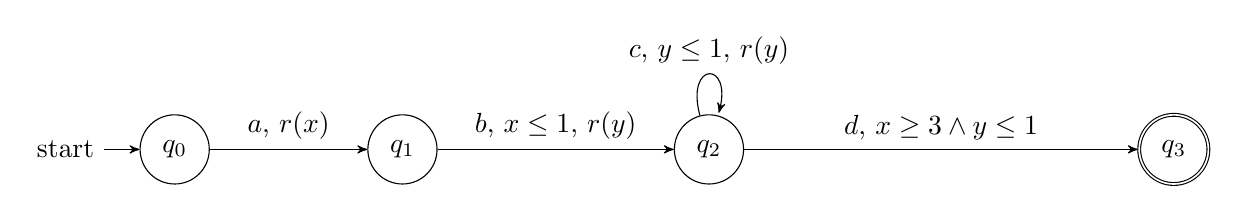
\begin{tikzpicture}[>=stealth']
  \node[state, initial] (q0) {$q_0$};
  \node[state] (q1) [right=2cm of q0] {$q_1$};
  \node[state] (q2) [right=3cm of q1] {$q_2$};
  \node[state, accepting] (q3) [right=5cm of q2] {$q_3$};
  \path[->]
  (q0) edge node[anchor=center, above] {$a$, $r(x)$} (q1)
  (q1) edge node[anchor=center, above] {$b$, $x \leq 1$, $r(y)$} (q2)
  (q2) edge [loop above] node[anchor=center, above] {$c$, $y \leq 1$, $r(y)$} ()
       edge node[anchor=center, above] {$d$, $x \geq 3 \land y \leq 1$} (q3);
\end{tikzpicture}
\end{figure}

\begin{definition}
  Трассировка $\tau$ -- последовательность пар $\{\left( a, t \right)\}$, 
  где $t \in \mathbb{N}$ -- задержка между предыдущим и текущим событиями, $a \in \Sigma$ -- символ перехода.
\end{definition}

\begin{definition}
  Значение $\nu(x) \in \mathbb{N}$ таймера $x \in C$ -- функция от таймера $x$.
\end{definition}

\begin{definition}
  Путь во временном автомате по трассировке $\{\left( a_i, d_i \right)\}$ -- последовательность из пар $\{\left( q_i, \nu_i \right)\}$ таких, 
  что $q_i \in Q$ -- состояние на шаге $i$, $\nu_i$ -- значения таймеров на шаге $i$, для которых выполняются следующие ограничения:
  \begin{itemize}
    \item $q_{2i} = q_{2i+1}$;
    \item $\forall x \in C: \nu_{2i+1}(x) - \nu_{2i}(x) = d_i$;
    \item $\exists! \langle q^1, q^2, a, g, R \rangle \in \Delta$: 
      \begin{itemize}
	\item $q_{2i+1} = q^1$;
	\item $q_{2i+2} = q^2$;
        \item $\forall x \in R: \nu_{2i+2}(x) = 0$;
	\item $\forall x \not\in R: \nu_{2i+2}(x) = \nu_{2i+1}(x)$;
	\item $\forall x \in C: \nu_{2i+1}(x)$ удовлетворяет $g$.
      \end{itemize}
  \end{itemize}
\end{definition}

Другими словами, в пути во временном автомате каждая пара из состояния и значений таймеров с 
четным номером отличается от предыдущей изменением состояния автомата, а также, возможно, сбрасыванием некоторого числа таймеров, 
каждая же пара с нечетным индексом отличается от предыдущей только увеличением значений таймеров.

\begin{example}
  Путем для трассировки $\{ \left( a, 10 \right) \left( b, 1 \right) \left( c, 1 \right) \left( c, 1 \right) \left( d, 1 \right) \}$
  будет являться последовательность: 
  \begin{equation}
    \begin{split}
      \{ &\left( q_0, \{ \nu_1 = 0, \nu_2 = 0 \} \right), \left( q_0, \{ \nu_1 = 10, \nu_2 = 10 \} \right), \left( q_1, \{ \nu_1 = 0, \nu_2 = 10 \} \right), \\
	 &\left( q_1, \{ \nu_1 = 1, \nu_2 = 11 \} \right), \left( q_2, \{ \nu_1 = 1, \nu_2 = 0 \} \right), \left( q_2, \{ \nu_1 = 2, \nu_2 = 1 \} \right), \\
	 &\left( q_2, \{ \nu_1 = 2, \nu_2 = 0 \} \right), \left( q_2, \{ \nu_1 = 3, \nu_2 = 1 \}  \right), \left( q_2, \{ \nu_1 = 3, \nu_2 = 0 \} \right), \\
         &\left( q_3, \{ \nu_1 = 4, \nu_2 = 1 \} \right) \}
    \end{split}
  \end{equation}
\end{example}

\begin{definition}
  Детерминированный временной автомат $\mathcal{A}$ -- временной автомат, для которого не существует трассировки, для которой существует два пути в данном временном автомате.
  \label{DTA}
\end{definition}

В дальнейшем, если это не оговорено заранее, под понятием временного автомата будет подразумеваться детерминированный временной автомат.

\begin{definition}
  Языком $\mathcal{L}(\mathcal{A})$ временного автомата $\mathcal{A}$ назовем множество всех принимаемых им трассировок.
\end{definition}

\begin{definition}
  Класс автоматов $\mathbb{K}$ называется достижимым за полином, если существует полином $p$, такой что для любых
  $\mathcal{A} \in \mathbb{K}, q \in Q_{\mathcal{A}}$ существует трассировка $\tau$ такая, что порожденный ей путь заканчивается в $q$ и $|\tau| < p(|\mathcal{A}|)$.
\end{definition}

Приведем также определения более слабого класса временных автоматов -- автоматов реального времени.

\begin{definition}
  Автомат реального времени -- временной автомат, такой что $C = \{c_0\}, R_{\delta} = \{c_0\}$ для любого перехода $\delta \in \Delta$.
  \label{rti}
\end{definition}

\begin{definition}
  Вероятностный детерминированный автомат реального времени -- кортеж $\langle \mathcal{A}, \mathcal{E}, \mathcal{T}, \mathcal{H} \rangle$, где
  \begin{itemize}
    \item $\mathcal{A} = \langle \Sigma, Q, q_0, C, \Delta, F \rangle$ -- автомат реального времени;
    \item $\mathcal{E}: Q \times \Sigma \rightarrow [0, 1]$ -- распределение вероятностей на множестве символов перехода;
    \item $\mathcal{T}: Q \times \mathcal{H} \rightarrow [0, 1]$ -- распределение вероятностей на множестве времен ожидания для данного интервала $h \in \mathcal{H}$;
    \item $\mathcal{H}$ -- конечное множество неперекрывающихся интервалов.
  \end{itemize}
  \label{rti++}
\end{definition}

\section{Теоретические результаты}
Следующие результаты были получены авторами статьи~\cite{1-dta}.

\begin{lemma}
  Класс временных автоматов не является достижимым за полином.
  \label{unreachable_lemma}
\end{lemma}

Лемма~\ref{unreachable_lemma} фактически утверждает, что, чтобы однозначно правильно синтезировать 
автомат по примерам, необходимо в качестве примеров иметь также пример экспоненциальной длины от размера временного автомата.

\begin{definition}
  Класс автоматов $\mathbb{K}$ называется различимым за полином, если существует полином $p$, такой что для любых
  $\mathcal{A}, \mathcal{A'} \in \mathbb{K}, \mathcal{L}(\mathcal{A}) \neq \mathcal{L}(\mathcal{A'})$ существует трассировка $\tau$, такая что 
  $\tau \in \mathcal{L}(\mathcal{A}) \Delta \mathcal{L}(\mathcal{A'})$ и $|\tau| < p(|\mathcal{A}| + |\mathcal{A'}|)$
\end{definition}

\begin{lemma}
  Класс временных автоматов не различим за полином.
  \label{distinguishability_lemma}
\end{lemma}

\begin{definition}
    Характеристическим множеством языка $\mathcal{L}_t$ для алгоритма $A$ называется множество трассировок $S_{cs} = \{S_{cs+}, S_{cs-}\}$, где
  $S_{cs+} \subseteq \mathcal{L}_t$, $S_{cs-} \subseteq \mathcal{L}_t^c$, такое что 
  для любого $S \supseteq S_{cs}, S_+ \subseteq \mathcal{L}_t, S_- \subseteq \mathcal{L}_t^c$ алгоритм $A$ на вход $S$ вернет автомат $\mathcal{A}$ такой, что $\mathcal{L}(\mathcal{A}) = \mathcal{L}_t$.
\end{definition}

\begin{definition}
  Класс автоматов $\mathbb{K}$ является эффективно синтезируемым в пределе (identifiable in the limit), если существуют полиномы $p, q$ и алгоритм $A$ такие, что
  \begin{itemize}
    \item время работы алгоритма на входе $S$ ограничено сверху полиномом $p(\mathop{\sum}\limits_{\tau \in S}|\tau|)$;
    \item для любого языка $\mathcal{A} \in \mathbb{K}$ существует $S_{cs} $ 
      -- характеристическое множество языка $\mathcal{A}$ для алгоритма $A$, такой что $\mathop{\sum}\limits_{\tau \in S_{cs}}|\tau| < q(|\mathcal{A}|)$.
  \end{itemize}
\end{definition}

\begin{theorem}
  Класс временных автоматов не является эффективно синтезируемым.
  \label{efficient_synthesis_theorem}
\end{theorem}

Доказаны также более сильные варианты данной теоремы.

\begin{theorem}
  Если $coNP \neq PSPACE$, то временной автомат не может быть эффективно синтезирован.
  \label{coNPneqPSPACE_lemma}
\end{theorem}

\begin{theorem}
  Если $NP \neq PSPACE$, то временной автомат не может быть эффективно синтезирован.
  \label{NPneqPSPACE_lemma}
\end{theorem}

Хоть и было доказано, что класс временных автоматов в целом не является эффективно синтезируемым, из него возможно выделить подкласс временных автоматов, 
который бы являлся эффективно синтезируемым. Приведем формулировку теоремы, которая немного проясняет ситуацию с временными автоматами.

\begin{theorem}
  Класс временных автоматов, в котором используется два или больше таймеров, не может быть эффективно синтезирован.
  \label{two_or_more_timers_lemma}
\end{theorem}

Таким образом, возможно, стоит обратить внимание на подкласс временных автоматов, которые могут использовать всего один таймер? 
В статье~\cite{1-dta} были также доказаны следующие факты:

\begin{lemma}
  Класс временных автоматов с одним таймером является полиномиально достижимым.
  \label{reachability_1_lemma}
\end{lemma}

\begin{lemma}
  Класс временных автоматов с одним таймером является полиномиально различимым.
  \label{distinguishability_1_lemma}
\end{lemma}

\begin{theorem}
  Класс временных автоматов с одним таймером является эффективно синтезируемым.
  \label{efficient_synthesis_1_theorem}
\end{theorem}

В качестве доказательства теоремы~\ref{efficient_synthesis_1_theorem} авторы статьи~\cite{1-dta} предоставили алгоритм ID-DTA-1, который эффективно синтезирует временной автомат в пределе.

\section{Эффективный синтез временного автомата с одним таймером с помощью алгоритма ID-DTA-1}

Впервые данный алгоритм был описан в статье~\cite{1-dta}. Идея алгоритма весьма проста.
Он руководствуется правилом: если меня ничто не останавливает от совершения следующего действия, то я его совершу. 
Пусть имеется некоторый минимальный автомат, который необходимо синтезировать по трассировкам. 
Алгоритм будет строить автомат итеративно. Построение начинает с одного стартового состояния. 
За одну итерацию к существующему автомату будет добавляться либо один новый переход, либо новое состояние и переход в него.
Значительное правило, которое используется в алгоритме: для любой числовой характеристики всегда существует строгий порядок перебора ее значений,
не зависящий от множества переданных алгоритму трассировок. Данное свойство необходимо для доказательства существования характеристического множества.

Каждая итерация алгоритма начинается с определения состояния, из которого будет выходить следующий переход. Процедура заключается в переборе состояний в порядке их появления в текущем автомате.
Выбирается первое состояние, для которого существует множество трассировок $T_q$, путь которых нужно продолжить из состояния $q$, то есть некоторый префикс путей трассировок
заканчивается в данном состоянии $q$ и не существует корректного перехода
далее по автомату. Теперь алгоритм выбирает символ перехода для нового ребра. Алгоритм перебирает символы перехода в лексикографическом порядке и выбирает первый символ $a$, для которого
во множестве $T_q$ существует трассировка, для продолжения пути которой по автомату требуется новый переход по символу $a$ из состояния $q$. Как видно, перебор состояний и перебор
символов перехода не зависит от множества трассировок: их алгоритм осуществляет всегда в одном и том же порядке. Единственное, на что влияет множество трассировок -- это значение, которое выбирается
первым. Далее для ребра алгоритму необходимо определить ограничения перехода. Для этого необходимо определить его верхнюю и нижнюю границы. Сначала определим верхнюю границу.
Верхняя граница перебирается сверху вниз, и выбирается первая, которая при выборе не внесет в автомат недетерминизм. Перебор всех возможных верхних границ слишком дорогостоящая операция из-за
того, что границы записываются, как минимум, в бинарном виде, и их перебор может быть экспоненциальным по отношению к размеру автомата. Поэтому алгоритм помнит для каждого состояния $q$ и символа
перехода $a$ предыдущую нижнюю границу $c'_{q, a}$. Тогда для нового перехода верхняя граница будет равна $c'_{q, a} - 1$. Изначально $c'_{q, a} = \infty$. Нижнюю границу, наоборот, он
перебирает снизу вверх, но по тем же причинам делать напрямик слишком плохая затея. Очевидно, что достичь того же эффекта можно используя множество $T_q$. Выбирая очередную границу множество $T_q$ делится
на две части: множество трассировок, которые будут проходить по данному ребру, и множество трассировок, которые, наоборот, проходить не будут. Чем ниже выбирается граница, тем большим становится
первое множество, причем трассировки при понижении границы могут переходить только из второго множества в первое. Это означает, что как только в первое множество будет добавлена трассировка,
которая ведет к неконсистентности в автомате, дальнейшее понижение границы не будет иметь смысла. Также нужно иметь ввиду, что нижнюю границу всегда можно опускать хотя бы до того момента, 
пока множества остаются неизменными. Значит нижняя граница точно равна значению таймера, увеличенному на единицу, в пути некоторой трассировки из $T_q$. Таким образом, алгоритм перебирает 
значения таймеров, увеличенных на единицу, трассировок в $T_q$, которым необходимо возникновение нового перехода с символом перехода $a$, делит эти трассировки на два множества, 
проверяет для первого множества условие на консистентность, из всевозможных вариантов значений выбирает наименьшее и присваивает его нижней границе. Далее определяется, нужно ли 
сбрасывать таймер после прохождения по синтезируемому переходу. В алгоритме таймер будет во множестве сброса, если при сбросе удастся получить интервал для ограничения не меньше, чем
интервал для ограничения без сброса. Осталось выбрать вершину, в которую будет вести данный переход. Здесь все просто: также перебираются состояния в порядке появления их в автомате и
выбрается первое, при проведении перехода в которое не образуется неконсистентности. Возможна также ситуация, когда такого состояния не существует. Тогда алгоритм добавляет новое состояние и проводит 
переход в него. Проверка на консистентность, упомянутая до этого, происходит не совсем обычным образом. Недостаточно просто проверить, в каких состояниях заканчиваются трассировки, ведь бывают
трассировки, для которых ещё не существует перехода, чтобы продолжить путь по автомату. Опасны две трассировки, которые в некоторый момент выравнивают значения таймеров и дальше переходят
по одинаковым символам, ожидая одинаковое время. Таким образом, алгоритм ID-DTA-1 проверяет существование двух трассировок $\tau(a, t)\tau''$ и $\tau'(a, t + \nu - \nu')\tau''$, для
которых пути для $\tau$ и $\tau'$ заканчиваются в состоянии $q$, имея значения таймеров $\nu$ и $\nu'$ соответственно. 

Теперь разберем, как можно построить для данного алгоритма характеристическое множество, зная минимальный временной автомат, который нужно синтезировать алгоритму ID-DTA-1. Характеристическое
множество будет строиться итеративно. Пусть на данной итерации уже имеется некоторое множество трассировок $S$ и текущий временной автомат $A$, который является частью минимального временного
автомата. Зная текущий автомат и характеристическое множество, можно легко определить, какой переход будет добавлен следующим в текущий автомат. 
Пусть он будет равен $\langle q, q', a, \left[ c'', c' \right], r \rangle$.  Если добавляемый переход не является частью минимального временного автомата, 
то нужно подкорректировать множество трассировок, чтобы оно запретило данный переход. 
Конкретнее, в данном переходе могут быть неверные границы перехода $g$, состояние $q'$, в которое ведет переход, и множество сбросов $r$.

Предполагая, что минимальный автомат является полным, то есть из каждого состояния можно перейти с любым значением таймера, в минимальном автомате существует переход с выбранной в текущем
автомате верхней границей $c'$ для нового перехода. Некорректной может быть лишь нижняя граница. Но в алгоритме граница $c''$ выбирается наименьшей из возможных, которые не приводят к неконсистентности.
Значит нужно предоставить две новые трассировки, которые бы привели к неконсистентности, проходя по новому переходу. Если $t \in r$, то добавим в множество трассировок
следующие трассировки: $\tau(a, c - \nu_{min})\tau'$, $\tau(a, c - \nu_{min} - 1)\tau')\tau'$, где $\tau$ -- трассировка, путь которой заканчивается в состоянии $q$ с наименьшим значением таймера 
$\nu_{min}$, которая существует и имеет полиномиальную длину~\ref{reachability_1_lemma}, $c > c''$ - нижняя граница соответствующего перехода в минимальном автомате. 
Если в минимальном автомате существует разделение на два ребра: одно, которое имеет нижней границей 
ограничения $c$, второе -- которое имеет верхней границей ограничения $c - 1$, то для множеств $\mathbb{L}_1 = \{\tau'' | \tau(a, c - \nu_{min})\tau'' \in \mathbb{L}_t \}$
$\mathbb{L}_2 = \{\tau'' | \tau(a, c - \nu_{min})\tau'' \in \mathbb{L}_t \}$, где $\mathbb{L}_t$ -- язык минимального автомата, выполняется $\mathbb{L}_1 \neq \mathbb{L}_2$. 
Иначе можно было бы слить два данных ребра и минимальный автомат бы таковым не являлся. Выберем $\tau': \tau' \in \mathbb{L}_1, \tau' \not\in \mathbb{L}_2$ или наоборот. 
Трассировка $\tau'$ существует и имеет полиномиальную длину по теореме~\ref{distinguishability_1_lemma}. Аналогично, при $t \not\in r$ нужно добавить трассировки $\tau(a, c - \nu_{min})(b, t_1)\tau'$ и
$\tau(a, c - \nu_{min} - 1)(b, t_1 + 1)\tau'$, чтобы создать неконсистентность при выборе нижней границы, меньшей чем $c$.

Чтобы устранить ненужный сброс, можно использовать трассировки $\tau(a, c - \nu_{min})\tau'$ и $\tau(a, c - \nu_{min} + 1)\tau'$, а чтобы, наоборот, установить сброс -- трассировки
$\tau(a, c - \nu_{min})(b, t_1)\tau'$, $\tau(a, c - \nu_{min} + 1)(b, t_1 - 1)\tau'$.

Если состояние $q'$, в которое ведет переход, не равно состоянию $q''$, в которое ведет соответствующий переход в минимальном автомате, добавим в характеристическое множество следующие трассировки: одну
принимаемую, другую отвергаемую:
$\tau(a, c - \nu_{min})(b, t_1)\tau''$ и $\tau'(b, t_1')\tau''$, где путь трассировки $\tau$ заканчивается в состоянии $q$, $\tau'$ -- в состоянии $q'$, $\nu' + t_1' = \nu + t_1 + c - \nu_{min}$,
$\nu, \nu'$ -- значения таймеров в конце путей $\tau$ и $\tau'$ соответственно. Таким образом, если алгоритм проведет переход в $q'$, он столкнется в неконсистентностью временного автомата.
Такие трассировки существуют, иначе минимальный автомат не является минимальным хотя бы по числу переходов.

Алгоритм ID-DTA-1 нужно воспринимать просто, как алгоритм приведенный в доказательство теоремы~\ref{efficient_synthesis_1_theorem}. Его скорость работы и эффективность, а также, возможно,
плохие характеристические множества, не позволяют генерировать хорошие временные автоматы. В поисках эффективного алгоритма, авторам приходится еще сильнее ограничить класс автоматов.

\section{Эффективный синтез автомата реального времени с помощью алгоритма RTI}

Данный алгоритм основан на адаптации одного из лучших алгоритмов синтеза конечных детерминированных автоматов EDSM~\cite{state-merging-dfa}. 
Он начинает синтез автомата с построения префиксного дерева трассировок. Префиксное дерево будет выступать в качестве первоначального автомата.
Далее алгоритм пытается находить состояния, которые, как он предполагает, являются одинаковыми в минимальном конечном автомате, и сливать их.

EDSM синтезирует автомат в так называемой красно-синей структуре. Данная структура представляет собой ни что иное, как разделение множества всех состояний на
множество красных состояний, которые являются уже просмотренными, множество синих состояний, которые сейчас рассматриваются, и множество непокрашенных
состояний, которые на данном шаге не рассматриваются. Красные состояния получаются окаймлены синими, то есть
для каждого синего состояния на текущем шаге есть красное состояние с ребром, которое ведет в него.

На каждом шаге выбирается один из двух вариантов: слить два состояния, либо покрасить синее состояние в красное. Слить можно либо два синих состояния,
либо красное состояние с синим. Предполагается, что между двумя красными состояниями переходы никаким образом поменяться не могут. При слиянии двух состояний 
множества переходов, выходящих из этих двух состояний, объединяются. Из-за этого получившийся автомат может оказаться недетерминированным: из новой вершины,
слитой из двух, могут выходить два ребра с переходом по одному и тому же символу. Данная проблема решается слиянием вершин, в которые ведут данные ребра. Тогда
два ребра, из-за которых образуется недетерминизм, также сливаются в одно. Но не всегда два состояния можно слить, иначе бы всегда получался автомат из одной вершины.
Предикатом на возможность слияния двух вершин будет то, что сливаемые вершины не должны быть разными по принятию трассировок (одна -- принимающей, вторая -- отвергающей), а также, 
если произошла ситуация недетерминизма, все потомки, которые необходимо слить, также должны удовлетворять предикату на возможность слияния.
Возможна так же ситуация, что на текущем шаге лучше покрасить синию вершину в красную, чем сливать вершины.

Нужно упомянуть, что синтез автомата в красно-синей структуре не ограничивает в возможности найти корректный минимальный автомат, ведь в некоторый момент каждая из вершин становится
синей и именно в этот момент необходимо корректно определить, нужно ли её слить с какой-то посещенной вершиной или же наоборот пропустить, чтобы потом слить с какой-нибудь
ещё непосещенной вершиной. Таким образом, размер автомата, который получится в конце, определяется стратегией, которую выбирают при синтезе автомата.
Так как абсолютно правильную стратегию сливаний и перекрасок выбрать сложно из-за того, что задача синтеза минимального детерминированного конечного автомата по трассировкам 
NP-полна~\cite{dfa-completeness}, то для этого применяют эвристики. В алгоритме EDSM используется эвристика для оценки правильности некоторой операции. Эта оценка является просто натуральным
числом. На текущей итерации оценивают правильность всевозможных слияний, всевозможных покрасок и применяют ту операцию, для которой оценка является наивысшей величиной среди остальных.
В качестве оценки обычно выступает оценка качества автомата, который получается после применения данной операции.
В EDSM обычно применяют следующую эвристическую оценку:

\begin{equation}
  pure = \#pos + \#neg
  \label{heur_1}
\end{equation}

В эвристике~\ref{heur_1} $\#pos$, $\#neg$ -- число слитых вершин, которые обе были принимающими и отвергающими соответственно. При равенстве нескольких наилучших оценок выбирают сначала
слияние, а затем покраску. Иными словами, с данной эвристикой у покраски всегда оценка правильности равна нулю. Таким образом, она будет произведена только в случае, 
если больше не осталось вершин, которые можно было бы слить. В качестве вершины для покраски можно выбирать любую.

Авторы алгоритма RTI~\cite{rti} адаптировали алгоритм EDSM, чтобы он мог использовать время. Авторам статьи для этого пришлось добавить в исходный алгоритм еще одну операцию -- разделение.
Изначально строится такое же префиксное дерево, как и в EDSM, без учета временных составляющих трассировок, и каждому переходу в префиксном дереве выставляются максимальные ограничения на переход.
При таком подходе некоторые трассировки могли попасть в префиксном дереве в одну и ту же вершину, хотя, возможно, одна из них являлась принимаемой, а другая -- отвергаемой. Таким образом, временной
автомат изначально не всегда является консистентным. Но в конце алгоритма он должен быть таковым. Так как, как и алгоритм EDSM, RTI работает в красно-синей структуре, и между красными состояниями
переходы не меняются, то необходимо, чтобы на каждом шаге красная часть автомата была консистентной, а также чтобы остальную часть автомата можно было превратить в консистентную
операциями слияния, разделения и перекраски. Изначальную неконсистентность исправляют операциями разделения. Возможно провести разделение только тех ребер, которые ведут из красных состояний в синие. 
При разделении ребра крайне нежелательно, чтобы два новых ребра вели в то же самое состояние, так как в таком случае это никак не избавит от неконсистентности.
Решается эта проблема глубоким копированием всего, куда ведёт резделяемое ребро. Это можно сделать потому что, всё, до чего можно добраться, проходя по разделяемому ребру, это либо синее, либо
непокрашенное состояние. То есть, на самом деле, это префиксное дерево из непокрашенных вершин. Поэтому из него нет ребер в красные состояния, и данную часть автомата можно без опасений скопировать.
Разделение ещё применяют в качестве вспомогательной операции при слиянии. Заметим, что так как разделение можно применить только на ребрах из красных состояний в синие, ребра, выходящие из синих
вершин, являются нетронутыми, а значит имеют изначальные максимальные ограничения на переход. Поэтому, перед тем как слить синее состояние с красным, алгоритм RTI разбивает ребра, 
выходящие из синего состояния, в тех же пропорциях, в которых находятся ребра, выходящие из красной вершины. В данном случае также применяется глубокое копирование выходящих префиксных деревьев.
Проверка на то, что автомат можно достроить до консистентного, точно такая же, как и в алгоритме EDSM (предикат на возможность слияния).

Аналогично, нужно упомянуть, что добавленная операция разделения не повлияет на возможность нахождения минимального временного автомата: необходимо в момент, когда состояние, из которого
выходят ребро, стало красным, а значит состояние, в которое входит, стало синим, провести правильное число разделений данного ребра в корректных местах. Но на практике у операции
разделения куда меньший приоритет по сравнению с операцией слияния, так как при слиянии как раз и произойдёт, скорее всего, самое правильное разбиение ребер. 

В алгоритме RTI точно так же применяется некоторое множество эвристических оценок. Первая из них -- это эвристика \ref{heur_1}, заимствованная из алгоритма EDSM. 
Видно, что операция разделения при данной эвристической оценке автомата может только его ухудшить, что не всегда правда. 

При равенстве нескольких наилучших оценок операций при применении любой эвристики приоритет отдается сначала слиянию, затем разделению, а затем покраске.

Следующая эвристика -- это подправленная эвристика \ref{heur_1}. В отличие в неё в данной эвристике также учитывается число новых неконсистентных состояний.

\begin{equation}
  consistent = \#pos + \#neg - \#posneg
  \label{heur_2}
\end{equation}

В эвристике~\ref{heur_2} $\#pos$, $\#neg$ -- также число слитых вершин, которые обе принимающие или отвергающие, $\#posneg$ -- число вершин, которые являются неконсистентными, то есть
существуют минимум две трассировки, одна из которых принимаемая, другая отвергаемая, которые заканчиваются в данном состоянии.

Следующая эвристика уже не является столь простой, но она по сути является расширением предыдущей эвристики, а именно расширяется понимание $\#posneg$. Ведь интуитивно кажется, что
если трассировки, ведущие в неконсистентное состояние имеют, большие разбросы по времени, то их легко разделить, и они не должны вносить сильный отрицательный вклад. А вот такие же строки,
которые имеют практически одинаковые времена на пути к неконсистентному состоянию, должны давать, наоборот, большой отрицательный вклад.
Таким образом, в этой эвристике особый упор отдается времени. Для каждых двух путей до листьев в префиксном дереве (временных строк), 
для которых одинаковы последовательности событий без времен, считается их похожесть. Так как их последовательности событий без времен одинаковы, они заканчиваются в одном и том же листе 
префиксного дерева. Похожесть двух строк определяется как вероятность того, что данные строки можно разделить, разделив равновероятно одно из ребер на пути от корня до листа, выбрав в качестве
времени для разделения временного ограничения равновероятно любую его точку. Эвристика выглядит следующим образом:

\begin{equation}
  \begin{split}
    impact = \mathop{\sum}\limits_{q \in Q_r}pure(q) - \mathop{\sum}\limits_{\tau \in \Delta_b}max\{impact(\tau, \tau') | \tau \in S^\delta_+ \land \tau' \in S^\delta_-\}& \\
						     + \mathop{\sum}\limits_{\tau \in \Delta_b}max\{impact(\tau, \tau') | \tau \in S^\delta_+ \land \tau' \in S^\delta_+\}& \\ 
						     + \mathop{\sum}\limits_{\tau \in \Delta_b}max\{impact(\tau, \tau') | \tau \in S^\delta_- \land \tau' \in S^\delta_-\}&
  \end{split}
  \label{heur_3}
\end{equation}

В эвристике~\ref{heur_3} $impact(\tau, \tau')$ -- похожесть двух временных строк $\tau$ и $\tau'$, $pure(q)$ -- эвристическая оценка EDSM только для вершины $q$, 
$S^\delta_+$, $S^\delta_-$ -- принимаемые и отвергаемые трассировки соответственно, которые в своем пути по текущему автомату проходят по ребру $\delta$.

Последняя эвристическая оценка тоже добавляет в изначальную оценку EDSM влияние неконсистентных вершин. В данном случае пытаются учесть величину того,
сколько потребуется разделений, чтобы избавить непокрашенные префиксные деревья от неконсистентных вершин. Так как точное число посчитать сложно из-за $NP$-трудности
данной задачи, применяется некоторый жадный алгоритм. Эвристическая оценка имеет следующий вид:

\begin{equation}
  splits = \mathop{\sum}\limits_{q \in Q}max(pure(q) - \#split(q), 0)
  \label{heur_4}
\end{equation}

В эвристике~\ref{heur_4} $\#splits(q)$ -- приблизительное число разделений, необходимых для избавления от неконсистентных состояний в префиксном дереве, выходящем из вершины $q \in Q$.

При тестировании лучше всего себя показали эвристические оценки \ref{heur_2} и \ref{heur_4}.

\section{Подход к синтезу в алгоритме Timed-k-Tail}

Данный алгоритм Timed-k-Tail~\cite{timed-k-tail} является адаптацией алгоритма k-Tail~\cite{k-tail}, применяемого для синтеза детерминированных конечных автоматов 
исключительно по позитивным примерам поведения. 
Алгоритм Timed-k-Tail нацеливается на генерацию автомата, хорошо описывающего поведение реальных программ. Предпологается, что есть некоторая эталонная программа, 
все трассировки которой являются корректными. Нужно построить некоторый автомат, имея только корректные трассировки, полученные при запусках данной программы, чтобы
можно было, в частности, валидировать корректность работы аналогичных программ. Трассировки для данного алгоритма тоже подойдут не любые.
События для данных трассировок делятся на два вида: начало некоторой функции и конец некоторой функции. Трассировка должна быть правильной скобочной последовательностью, если назначить 
начало функций в качестве открывающейся скобки, а конец в качестве закрывающейся скобки, причем у разных функций должны быть разные скобки.
Алгоритм делится на несколько стадий.

Первая стадия данного алгоритма -- нормализация. На вход изначально поступает некоторое множество трассировок выполнения реальной программы. Первое, что происходит в алгоритме, нормализация:
трассировки изменяются таким образом, чтобы время старта для каждой трассировки было одинаковым: обычно от каждого времени в трассировке отнимают время первого события
в данной трассировке, таким образом выходит, что первое событие каждой трассировки стартует в момент времени ноль. Однако все задержки времени между любой парой событий в трассировке
сохраняются неизменными. 

Вторая стадия -- построение по трассировкам префиксного дерева. В данном алгоритме используется огромное число таймеров, чтобы замерять задержки между началом функции в некоторый
момент времени и её концом. Также будет существовать один нулевой (глобальный) таймер $t$, который нельзя будет сбрасывать. Видоизменим трассировки. 
Во-первых, каждая трассировка теперь будет аннотироваться не временем, а ограничениями и множеством таймеров для сброса. В качестве первого ограничения для каждого события $j$ в трассировке $i$
добавим $t = time_{i, j}$, где $time_{i, j}$ -- момент времени, в который произошло событие $j$ в трассировке $i$. Далее для каждого события начала функции добавим во множество сброса новый
таймер. Пусть в трассировке $i$ для события $j$ этот таймер будет иметь номер $c$. Тогда в трассировке $i$ нужно найти событие конца данной функции, пусть оно по номеру равно $k$, и в его
аннотацию добавить ещё одно ограничение $c = time_{i, k} - time_{i, j}$. Таким образом замеряется время работы каждого запуска какой-либо функции. Последнее, что нужно сделать,
первому событию в каждой из трассировок добавить во множество сброса таймер $t$, таким образом позволяя не думать о том, какими таймеры могут быть в корне будущего префиксного дерева, все они всё равно
в будущем будут сброшены. И только после данных операций по видоизмененным трассировкам нужно построить префиксное дерево.

Третья стадия -- слияние состояний. На текущем этапе нужно выбрать величину $k$, присутствующую в названии данного алгоритма. Идея, которая главенствует на данной стадии синтеза автомата,
гласит, что <<скорее-всего>> система находится в одном и том же состоянии, если, как минимум, первые $k$ событий, исходящие из двух состояний, совпадают. Но нужно также разобраться с ребрами, которые
получаются при слиянии двух состояний. Алгоритм предписывает реберам, выходящим из сливаемых состояний с одинаковыми переходными символами, также слиться, при этом объединяя множества сбросов и
множество ограничений. 

Четвертая стадия -- улучшение таймеров. К текущему моменту у автомата может возникнуть много таймеров, которые меряют одно и то же из-за того, что на предыдущей стадии произошло слияние состояний.
На данном этапе нужно избавиться от таких таймеров. Пара таймеров меряет одно и то же, если каждый из них сбрасывается и проверяется на одних и тех же переходах. Находим все таймеры, которые меряют
одно и то же, и оставляем из данного множества только один, остальные удаляем из всего автомата.

Пятая стадия -- генерация ограничений. Чтобы автомат мог хоть что-то валидировать, необходимо расширить ограничения. На некоторых переходах в ограничениях таймер мог встречаться по несколько раз, 
например $t = 3 \land t = 5$. Понятно, что в текущем состоянии автомат ничего не способен принять. Поэтому на данной стадии заменяют все такие ограничения на одно таким образом, чтобы новое ограничение
включило в себя все или почти все предыдущие равенства. Возвращаясь к примеру, логично будет заменить равенства на новое ограничение $3 \leq t \leq 5$. Замена на самом деле определяется политикой.
В статье приводится два вида политик. Первая политика -- в качестве нового ограничения выбирать промежуток $[(1-\epsilon)min, (1+\epsilon)max]$, где $min$, $max$ -- минимальное
и максимальное значение чисел, встреченных в правых частях изначальных равенств. Вторая политика -- в зависимости от параметра $\gamma$
на основе изначальных равенств, выдать промежуток, куда попадут $\gamma$ возможных трассировок, в предположении, что изначальное распределение правых частей равенств было нормальным.

Данный алгоритм интересен своей простотой и нетребовательностью к разметке данных. Однако качество получаемых временных автоматов тоже не велико.

\section{Применение временных автоматов на практике. Алгоритм MOHA}

Некоторая модификация алгоритма RTI -- алгоритм RTI+~\cite{rti-plus}, умеющий генерировать вероятностные детерминированные автоматы реального времени (определение~\ref{rti++}),
опираясь только на принимаемые трассировки, используется в алгоритме MOHA~\cite{moha} как одна из составных частей реализации. Опишем алгоритм MOHA и применение в нем временных автоматов.

Данный алгоритм был применен на данных из двух открытых множеств траекторий NGSIM~\cite{ngsim}: I80 и US101. В данных множествах положение автомобилей обновляется с частотой 10Гц.
Алгоритм состоит из нескольких стадий: сначала происходит крупнозернистая грануляция примеров, затем символизированные примеры подаются на вход RTI+ в результате которого
появляется автомат, состояния данного автомата кластеризуются алгоритмом MISSI~\cite{moha}, образуя режимы в автомате, далее на данных режимах тренируются модели отслеживания
машин.

Чтобы можно было применить алгоритм RTI+, сначала данные необходимо сконвертировать данные в валидные. Для этого по имеющимся данным вычисляются переменные для любых
двух подряд идущих транспортных средств: скорость транспортного средства, относительное расстояние до впередиидущего транспортного средства, относительная скорость двух транспортных
средств и ускорение первого транспортного средства. Далее к полученным данным применяется алгоритм кластеризации K-means. Разные кластеры теперь обозначают разные символы перехода.
Новое событие происходит, когда значительно меняется состояние транспортного средства, следовательно изменяется кластер, к которому оно принадлежит. В качестве символа перехода берется номер
нового кластера. Символизированные таким образом примеры подаются на вход алгоритму RTI+.

По полученному автомату и поданным на его вход примерам формируются пути данных примеров по автомату. Отсечем от путей временную составляющую и, используя их, начнем кластеризовать состояния
для получния режимов. Извлечем из путей подпути длины не меньше заданной константы $L_{min}$ с встречаемостью чаще заданной константы $\epsilon$ и кластреризуем их по похожести. Режим для
состояний определяются путем голосования. То есть режимом для конкретного состояния будет являеться номер кластера, в котором подпути чаще всего его использовали.

По результатам тестирования было установлено, что представленный алгоритм значительно превосходит алгоритмы, представленные до него, что является хорошим показателем важности
использования временных автоматов в моделях машинного обучения и важности построения новых алгоритмов синтеза временных автоматов.

\section{Задача удовлетворимости булевых формул и задача удовлетворения ограничений}

Задача удовлетворимости булевых формул и задача удовлетворения ограничений являются известными NP-полными задачами. Одной из первых была доказана NP-полнота задачи удовлетворения
булевых формул. После этого доказательства NP-трудности и NP-полноты стали достаточно тривиальными: в первом случае нужно свести задачу удовлетворения булевых формул
к текущей задаче, а во втором случае -- в дополнение к первому нужно еще и предоставить обратное сведение. Из-за того, что вышеупомянутым задачи чаще всего используются для
доказательств NP-полноты, то было разработано большое количество пакетов программ, позволяющих их решать за хоть сколько-то разумное время. 

В частности к задаче удовлетворения булевых формул можно свести задачу построения минимального детерминированного конечного автомата.
Задача генерации минимального временного автомата представляет собой более сложную задачу из-за использования таймеров и ограничений на них.
Тем не менее она легко сводится к задаче удовлетворения ограничений.

%% Так помечается конец обзора.
\finishrelatedwork

\chapterconclusion

\begin{itemize}
  \item Даны основные определения и факты из предметной области. Произведен краткий анализ фактов.
  \item Изучены лучшие из существующих решений генерации временных автоматов.
  \item Произведен обзор существующих решений.
\end{itemize}

\chapter{Предлагаемый метод синтеза временного автомата на основе программирования в ограничениях}

\section{Постановка задачи}

На текущий момент существуют методы генерации временных автоматов в пределе, а также эвристические методы генерации временных автоматов, 
однако отсутствует попытка разработки алгоритма, генерирующего минимальный временной автомат на основе сведения к задаче удовлетворения ограничений.

Таким образом в данной работе решались следующие задачи:

\begin{itemize}
  \item Изучение возможностей программного пакета Minizinc~\cite{minizinc}, предназначенного для решения задач удовлетворения граничений. 
  \item Разработка сведения задачи к задаче удовлетворения ограничений.
  \item Реализация решения на основе сведения и сравнение с существующим решением.
\end{itemize}

\section{Переменные, используемые в решателе задачи удовлетворения ограничений}

Введем переменные, используемые при синтезе временного автомата:

\begin{itemize}
  \item $V$ -- число состояний, которые в данный момент использует решатель системы ограничений;
  \item $T$ -- число таймеров, которые используются во временном автомате;
  \item $E$ -- максимальная степень вершины, которая может использоваться в автомате;
  \item $M$ -- число ребер, используемое в префиксном дереве;
  \item $N = M + 1$ -- число вершин, используемое в префиксном дереве;
  \item $inf$ -- верхняя граница для ограничения на переходе. Обычно при синтезировании автомата с $n$ таймерами в качестве верхней границы выбирается максимальная сумма
    ожиданий переходов по каждой из трассировок, при синтезировании временного автомата RTA в качестве верхней границы выступает максимальное ожидание среди всех ожиданий
    каждой из трассировок;
  \item $TC$ -- максимальное число активных таймеров, которые можно использовать во временном автомате;
  \item $TE$ -- максимальное число переходов, которое можно использовать во временном автомате;
  \item $COL = \{ W, G, B \}$ -- множество цветов, в которые могут быть покрашены вершины префиксного дерева. $W$ обозначает, что в данном состоянии оканчивается отвергаемая
    трассировка, $B$ -- принимаемая, $G$ в свою очередь означает, что в данном состоянии не заканчивается ни одна из трассировок;
  \item $S$ -- множество используемых в трассировках событий;
  \item $labels: 1..M \rightarrow S$ -- события каждого из переходов $m \in 1..M$ в префиксном дереве;
  \item $next: 1..M \rightarrow 1..N$ -- состояния, из которого выходят переходы $m \in 1..M$;
  \item $prev: 1..M \rightarrow 1..N$ -- состояния, в которые идут переходы $m \in 1..M$;
  \item $times: 1..M \rightarrow 0..inf$ -- времена ожидания переходов $m \in 1..M$;
  \item $table: 1..V \times 1..E \rightarrow 1..V$ -- таблица переходов состояний: состояния, в которые переходят из состояния $v \in 1..V$ по переходу из данного состояния $e \in 1..E$;
  \item $symbols: 1..V \times 1..E \rightarrow S$ -- таблица переходов событий: события, необходимые для перехода из состояния $v \in 1..V$ по переходу из данного состояния $e \in 1..E$;
  \item $final: 1..V \rightarrow \{ False, True \}$ -- условия для каждого из состояний $v \in 1..V$, что оно является принимающим;
  \item $mn: 1..V \times 1..E \times 1..T \rightarrow 0..inf$ -- нижние границы ограничений для каждого из состояний $v \in 1..V$, каждого из переходов из данного состояния $1..E$ и каждого из
    таймеров $t \in 1..T$;
  \item $mx: 1..V \times 1..E \times 1..T \rightarrow 0..inf$ -- верхние границы огранчений для каждого из состояний $v \in 1..V$, каждого из переходов из данного состояния $1..E$ и каждого из
    таймеров $t \in 1..T$;
  \item $reset: 1..V \times 1..E \times 1..T \rightarrow \{ False, True \}$ -- условие для каждого из состояний $v \in 1..V$, каждого из переходов из данного состояния $e \in 1..E$,
    каждого из таймеров $t \in 1..T$, что данный таймер сбрасывается на данном переходе из данного состояния;
  \item $disTimer: 1..V \times 1..E \times 1..T \rightarrow \{ False, True \}$ -- условие для каждого из состояний $v \in 1..V$, каждого из переходов из данного состояния $e \in 1..E$,
    каждого из таймеров $t \in 1..T$, что данный таймер не используется на данном переходе из данного состояния;
  \item $disEdge: 1..V \times 1..E \rightarrow \{ False, True \}$ -- условие, что для каждого из состояний $v \in 1..V$, каждого из переходов из данного состояния $e \in 1..E$,
    что данное ребро не используется. То есть в автомате переходы, для которых условие выполняется, не существуют;
  \item $map: 1..N \rightarrow 1..V$ -- вершины из временного автомата, соответствующие вершинам из префиксного дерева;
  \item $after: 1..N \times 1..T \rightarrow 0..inf$ -- значения таймеров $t \in 1..T$ сразу после перехода по ребрам, ведущим в вершины $q \in 1..N$ префиксного дерева. Для корня префиксного
    дерева можно считать, что существует некоторое невыделяемое на рисунках ребро, по которому в него приходят;
  \item $before: 1..M \times 1..T \rightarrow 0..inf$ -- значения таймеров $t \in 1..T$ сразу перед переходом по ребрам $e \in 1..M$ префиксного дерева;
  \item $parents: 1..V \rightarrow 1..V$ -- вершины, из которых в первый раз попадают в соответствующие вершины $v \in 1..V$ при обходе автомата алгоритмом BFS;
  \item $minEdge: 1..V \rightarrow 1..E$ -- минимальные по номерам ребра, ведущие из родительских вершин в вершины $v \in 1..V$.
\end{itemize}

\section{Ограничения, используемые в решателе системы ограничений}

Приведем множество ограничений, используемых в решателе систем ограничений.

\subsection{Ограничения, запрещающие недетерминизм}

Исходя из определения~\ref{DTA} детерминированного временного автомата, не должно существовать трассировки, которая порождает два или более корректных пути по временному автомату.
То есть, не должно существовать трассировки, путь которой заканчивается в некотором состоянии с некоторым набором значений таймеров, и существует два перехода по разным ребрам,
удовлетворяя ограничения на данных ребрах. Но такого вида условие было бы слишком тяжелым для решателя систем ограничений. Запишем несколько более сильное, но менее общее, ограничение, запрещающее
недетерминизм.

\begin{lstlisting}[float=!h,language=Mzn,caption={Ограничение, запрещающее недетерминизм},label={nondeterminism}]
constraint
forall (s  in 1..V,
        e1 in 1..E,
        e2 in 1..E
  where e1 != e2)
(symbols[s, e1] = symbols[s, e2] -> 
 (disEdge[s, e1] \/
  disEdge[s, e2] \/
  exists (t in 1..T) 
  (mx[s, e1, t] < mn[s, e2, t] \/ 
   mx[s, e2, t] < mn[s, e1, t])));
\end{lstlisting}

В ограничении~\ref{nondeterminism} не допускается существование двух переходов по одному символу из одного состояния, для которых гиперпаралеллепипеды, составленные из ограничений каждого таймера,
пересекаются. Очевидно, чтобы недопустить пересечение гиперпаралеллепипедов необходимо иметь хотя бы один таймер, ограничения которого для первого и второго перехода не пересекаются, то есть
нижняя граница ограничения данного таймера на первом переходе больше чем на втором, или наоборот.

\subsection{Основной предикат на переходы}

Основной предикат -- предикат на то, что переходу в префиксном дереве соответствует данный переход в автомате.

\begin{lstlisting}[float=!h,language=Mzn,caption={Основной предикат на переходы},label={main_predicate}]
predicate check (1..M: pe, 1..E: e) =
 symbols[map[prev[pe]], e] = labels[pe] /\
 map[next[pe]] = table[map[prev[pe]], e] /\
 forall (t in 1..T)
 (before[pe, t] >= mn[map[prev[pe]], e, t] /\
  before[pe, t] <= mx[map[prev[pe]], e, t] /\
  after[next[pe], t] = if reset[map[prev[pe]], e, t] then 0 else before[pe, t] endif);
\end{lstlisting}

Чтобы переходу в префиксном дереве соответствовал переход в автомате, необходимо выполнение следующих условий:

\begin{itemize}
  \item символ перехода в префиксном дереве равен символу перехода в автомате;
  \item состоянию, из которого ведет переход префиксного дерева, соответствует состояние, из которого ведет переход автомата;
  \item состоянию, куда ведет переход префиксного дерева, соответствует состояние, куда ведет переход автомата;
  \item значения каждого из таймеров сразу до перехода удовлетворяют ограничениям перехода по каждому из таймеров;
  \item значения таймеров сразу после перехода в префиксном дереве равны значениям таймеров сразу перед переходом в случае,
    если таймеры не находятся во множестве сброса перехода, иначе равны нулю.
\end{itemize}

Применим описанный выше предикат дважды: необходимо, чтобы для каждого перехода из префиксного дерева существовал единственный
соответствующий ему переход в автомате, а также необходимо, чтобы для каждого перехода в автомате существовал как минимум один соответствующий
переход в префиксном дереве. Это описывают следующие ограничения:

\begin{lstlisting}[float=!h,language=Mzn,caption={Использование основного предиката},label={main_constraints}]
constraint
forall (pe in 1..M)
(exists (e in 1..E)
 (check (pe, e)));

constraint
forall (s in 1..V,
        e in 1..E)
(disEdge[s, e] \/
 exists (pe in 1..M)
 (map[prev[pe]] = s -> check (pe, e)));
\end{lstlisting}

\subsection{Стартовые ограничения}

Стартовыми ограничениниями будут являться:

\begin{itemize}
  \item корню префиксного дерева соответствует стартовая вершина в автомате. 
  \item значения всех таймеров сразу после перехода в стартовую вершину равны нулю.
\end{itemize}

\begin{lstlisting}[float=!h,language=Mzn,caption={Стартовые ограничения},label={start_constraint}]
constraint
forall (t in 1..T)
(after[1, t] = 0);

constraint
map[1] = 1;
\end{lstlisting}

\subsection{Ограничения на минимальность}

Основной минимальностью является число состояний данного автомата. Но состояния автомата перебираются вне решателя систем ограничений. Решатель только пытается удовлетворить
переданные ему ограничения. Остальные, менее важные минимальности -- минимальность на число переходов в данном временном автомата и минимальность количества
активных таймеров в автомате. Таймер активен на переходе автомата, если либо верхняя граница ограничения для данного таймера не равна $inf$, либо нижняя граница ограничения
для данного таймера не равна нулю. Таким образом, необходимые ограничения приведены на листингах~\ref{disabled_edges_min}~\ref{disabled_timers_min}

\begin{lstlisting}[float=!h,language=Mzn,caption={Стартовые ограничения-1},label={disabled_edges_min}]
constraint
constraint
sum  (s in 1..V,
      e in 1..E)
(1 - bool2int (disEdge[s, e])) <= TE;
\end{lstlisting}

\begin{lstlisting}[float=!h,language=Mzn,caption={Стартовые ограничения-2},label={disabled_timers_min}]
constraint
sum  (s in 1..V,
      e in 1..E,
      t in 1..T)
(1 - bool2int (disTimer[s, e, t] \/ disEdge[s, e])) <= TC;
\end{lstlisting}

Ограничение~\ref{disabled_edges_min} ограничивает число ребер, по которым проходят пути трассировок, которое не должно превосходить $TE$.
Ограничение~\ref{disabled_timers_min} ограничивает число активных таймеров, которое не должно превосходить $TC$.

\subsection{Ограничение на допускающие состояния}

Так как в решатель передается префиксного дерево, каждое из состояний которого покрашено в одно из трех цветов, автомат должен учитывать эту информацию при покраске своих вершин.
Вершина автомата может быть принимающей трассировки только в случае, если соответствующие ей состояния префиксного дерева имеют цвета либо $G$, либо $B$. Отвергающей же имеет право
быть только в случае, если соответствующие ей состояния префиксного дерева имеют цвета либо $G$, либо $W$. Запишем это в ограничениях:

\begin{lstlisting}[float=!h,language=Mzn,caption={Ограничения на допускающие состояния},label={term}]
constraint
forall (s  in 1..V,
        ps in 1..N)
(map[ps] = s -> (acc[ps] = B -> final[s]));

constraint
forall (s  in 1..V,
        ps in 1..N)
(map[ps] = s -> (acc[ps] = W -> (not final[s])));
\end{lstlisting}

То есть, если состоянию $ps$ префиксного дерева соответствует состояние $s$ автомата, а также состояние $ps$ покрашено в цвет $B$, то состояние $s$ обязано быть принимающим. То же
самое для цвета $W$ и отвергаемого состояния.

\subsection{Ограничения BFS}

Ограничения BFS впервые были представлены в работе~\cite{bfs}. Они позволяют значительно сократить область поиска нужного детерминированного конечного 
автомата за счет установления нумерации вершин в порядка обхода BFS. Для временных автоматов можно применить ту же самую идею.

Ограничения BFS представляют собой ограничения на порядок вершин и ограничения на порядок переходов. Ограничения на порядок вершин требует, чтобы состояния, в которые можно прийти
из меньших но номеру состояний, имели номер меньше, чем состояния, в которые можно прийти из больших по номеру состояний. Порядок на ребрах требует, чтобы состояния, в которые
ведут меньшие по номеру переходы, имели номер меньше, чем состояния, в которые ведут большие по номеру переходы.

Наложим ограничения на $parents$ и $minEdge$. В алгоритме BFS при обходе графа используется очередь. Соответственно, вершины, попавшие в очередь раньше, раньше извлекаются и получают меньший номер.
Причем после извлечения в конец очереди добавляются вершины по порядке просмотра ребер, которые ещё не были до этого в очереди, но в них можно перейти из только что извлеченной вершины по
соответствующему ребру. Тогда для данного состояния $a$ $parents[a]$ должно указывать на состояние $a'$, которое должно является наименьшим по номеру состоянием, из которого можно попасть в вершину,
а $minEdge$ должно указывать на наименьшее по номеру ребро, ведущее из $a'$ в $a$.
Следующее ограничение~\ref{bfs_1} накладывает описанные выше ограничения: для любого ребра меньше чем $minEdge[a]$ переход из $parents[a]$ ведет в отличную от $a$ вершину, а также из любого состояния
меньшего по номеру чем $parents[a]$ по любому переходу нельзя попасть в $a$.

\begin{lstlisting}[float=!h,language=Mzn,caption={BFS-ограничения-1},label={bfs_1}]
constraint
forall (s in 2..V)
(table[parents[s], minEdge[s]] = s /\
 forall (e in 1..E)
 (e < minEdge[s] -> table[parents[s], e] != s) /\
 forall (s1 in 1..V)
 (s1 < parents[s] ->
  forall (e in 1..E)
  (disEdge[s1, e] \/ table[s1, e] != s)));
\end{lstlisting}

Теперь необходимо добавить ограничение двух условий, описанных выше.

\begin{lstlisting}[float=!h,language=Mzn,caption={BFS-ограничения-2},label={bfs_2}]
constraint
forall (s1 in 2..V,
        s2 in 2..V
  where s1 < s2)
(parents[s1] < parents[s2] \/
 parents[s1] = parents[s2] /\
 minEdge[s1] < minEdge[s2]);
\end{lstlisting}

Единственное, что осталось сделать -- определить в каком порядке перебирать переходы. Ведь могут встречаться два переходы с одинаковыми символами или переходы с одинаковыми ограничениями.
Чтобы задать на них полный порядок, обычно перебирают каждый из параметров в некотором порядке и делают выбор минимального перехода лексикографически. В данном случае это можно сделать
следующим ограничением:

\begin{lstlisting}[float=!h,language=Mzn,caption={BFS-ограничения-3},label={bfs_3}]
constraint
forall (s in 1..V,
        e in 1..(E - 1))
(disEdge[s, e] -> disEdge[s, e + 1]);

constraint
forall (s in 1..V,
        e in 1..(E - 1))
((not disEdge[s, e]) -> 
 ((not disEdge[s, e + 1]) ->
  symbols[s, e] < symbols[s, e + 1] \/
  (symbols[s, e] = symbols[s, e + 1] /\
   exists (t in 1..T)
   ((mn[s, e, t] < mn[s, e + 1, t] \/
     (mn[s, e, t] == mn[s, e + 1, t] /\
      mx[s, e, t] < mx[s, e + 1, t])) /\
    forall (t0 in 1..T)
    (t0 < t ->
     mn[s, e, t0] == mn[s, e, t0] /\
     mx[s, e, t0] == mx[s, e, t0])))));
\end{lstlisting}

То есть можно сравнить переходы сначала по символу, затем по нижней границе первого таймера, затем по верхней границе второго таймера, затем по нижней границе второго таймера, затем
по верхней границе второго таймера и так далее. Первое ограничение в~\ref{bfs_3} тоже немного обрезает область поиска: все неактивные ребра будут находиться последними в списке ребер,
выходящих из данной вершины. Однако, последнее ограничение~\ref{bfs_3} является очень трудным для решателя систем ограничений, поэтому порой оно может быть опущено.

\subsection{Ограничения для автоматов реального времени}

Простой способ превратить алгоритм поиска n-DTA в алгоритм поиска автоматов реального времени -- передать в решатель в качестве $T = 1$, а также добавить ограничения:

\begin{lstlisting}[float=!h,language=Mzn,caption={Ограничения RTA},label={rta_constraints}]
constraint
forall (s in 1..V,
        e in 1..E,
        t in 1..T)
(reset[s, e, t]);
\end{lstlisting}

\section{Порядок генерации}
С генерацией минимальных временных автоматов дело обстоит несколько сложнее, чем с генерацией минимальных детерминированных конечных автоматов.
Первый признак того, что все не очень просто -- невозможность как-то разумно ограничить число выходящих переходов из вершины. Ведь в обычном детерминированном конечном автомате можно
было просто ограничить данное число мощностью алфавита символов переходов. В данной же задаче по одному и тому же символу перехода из данного состояния может выходить несколько
переходов, имея непересекающиеся гиперпаралеллепипеды возможных значений таймеров.
Далее приходит понимание того, что понятие минимальности само по себе довольно расплывчато. Рассмотрим следующий возможный случай. 
Пусть есть множество трассировок, в которых задержки во времени задаются сколь угодно точно. Тогда, если данные трассировки получились случайным образом,
очень вероятна ситуация, когда всевозможные задержки во времени будут различными. А это означает, что есть возможность сгенерировать автомат из двух состояний, принимающего и отвергающего,
и с огромным количеством переходов. Главная цель данного автомата -- направить трассировку по последнему переходу, так как безразлично, как она ведет себя до последнего перехода, ведь в
конце всё равно возможно будет их различить и направить в правильное состояние. Тогда можно понять, что в реальности можно встретить несколько валидных <<минимальных>> пар из количества
состояний и числа ребер, лежащих на Парето-фронте. 
Однако в отличии от количества состояний во временном автомате хорошим показателем его минимальности является количество ребер.

Основной алгоритм можно представить псевдокодом на листингах \ref{lst1}, \ref{lst2}. 
Алгоритм состоит из трех основных циклов. В цикле неосновном цикле, со строки~\ref{lst:line:start1} до строки~\ref{lst:line:end1}, производится производится заполнение и последующая сортировка
пар из числа состояний и степени вершины. Алгоритм перебирает число состояний и степень вершины в порядке увеличения числа переходов. 
Также алгоритм поддерживает внутри себя текущее множество трассировок (строка~\ref{lst:line:activeTraces}). Постепенно данное множество пополняется.
В втором цикле, со строки~\ref{lst:line:start2} до строки~\ref{lst:line:end2}, идет поиск первой пары из числа состояний и степени вершины,
для которой автомат построенный с такими характеристиками, по префиксному дереву, построенному из текущего множества трассировок (пример,
являлся бы консистентным со всеми трассировками. Если же построенный автомат не является консистентным со
всем множеством трассировок, то в текущее множество добавляется еще одна трассировка, которую построенный автомат не удовлетворил, и которая из таких является минимальной по длине.
После данного цикла два последующих цикла, со строки~\ref{lst:line:start3} до строки~\ref{lst:line:end3} и со строки ~\ref{lst:line:start4} до строки~\ref{lst:line:end4} соответственно,
пытаются минимизировать построенный автомат. Минимизация сначала происходит по числу переходов в данном автомате, а затем по числу активных таймеров.
Минимизация числа переходов нужна в том случае, если состояния имеют различную степень. Действуют два цикла одинаково: пытаются построить автомат с меньшей характеристикой чем имеющаяся и,
если то удается, новый автомат опять же проходит проверку на консистентность со всеми трассировками, так как при минимизации нужно не забывать, что главная цель -- удовлетворить все трасcировки.
Если новый автомат неконсистентен со всеми трассировками, то также в текущее множество добавляется минимальная неудовлетворимая. Данный подход хорош по причине того, что
в самом первом цикле алгоритм перебирает элементы из $\mathbb{N}^2$. А значит перед тем, как он найдет нужную пару придется отсечь много неправильных пар, что хотелось бы делать имея малое число
состояний в префиксном дереве. Причем, в алгоритм редко добавляются абсолютно все трассировки, самые длинные и часто удовлетворимые остаются нетронутыми.

\begin{example}
  Построим для множества трассировок $A$ префиксное дерево~\ref{prefix_tree}. 
\begin{equation}
  A = \{\{ \left( a, 1 \right) \left( c, 3 \right) \}, \{ \left( b, 2 \right), \left( d, 4 \right), \left( f, 6 \right) \}, \{ \left( b, 2 \right), \left( c, 5 \right) \}, \{ \left( b, 2 \right) \}\}
\end{equation}
\begin{figure}[!h]
\caption{Пример префиксного дерева}\label{prefix_tree}
\centering
\begin{tikzpicture}[>=stealth', node distance=3cm]
  \node[state, initial] (q0) {$q_0$};
  \node[state] (q1) [below left of=q0] {$q_1$};
  \node[state, accepting] (q2) [below right of=q0] {$q_2$};
  \node[state, accepting] (q3) [below left of=q1] {$q_3$};
  \node[state] (q4) [below left of=q2] {$q_4$};
  \node[state, accepting] (q5) [below right of=q2] {$q_5$};
  \node[state, accepting] (q6) [below of=q4] {$q_6$};
  \path[->]
  (q0) edge node[anchor=center, above left] {$a, 1$} (q1)
       edge node[anchor=center, above right] {$b, 2$} (q2)
  (q1) edge node[anchor=center, above left] {$c, 3$} (q3)
  (q2) edge node[anchor=center, above left] {$d, 4$} (q4)
       edge node[anchor=center, above right] {$e, 5$} (q5)
  (q4) edge node[anchor=center, left] {$f, 6$} (q6);
\end{tikzpicture}
\end{figure}
\end{example}

\chapterconclusion

В данной главе была описана и разъеснена идея решения, описано и разъеснено сведение к задаче удовлетворения ограничений (основные сущности и ограничения).


\begin{algorithm}[!h]
\caption{Псевдокод алгоритма}\label{lst1}
\begin{algorithmic}[1]
	\Function{Основной алгоритм}{$traces$, $timersNumber$}
		\State $order \gets []$
		\For{$states \gets [1; \infty]$} \label{lst:line:start1}
			\For{$vertexDegree \gets [1; \infty]$}
				\State $order \mathrel{+}= \left(states, vertexDegree\right)$
			\EndFor
		\EndFor	\label{lst:line:end1}
		\State Отсортировать $order$ по величине $states * vertexDegree$
		\State $activeTraces \gets []$ \label{lst:line:activeTraces}
		\State $activeTraces \mathrel{+}=$ минимальная трассировка из $traces$ по длине
		\State $states \gets 0$
		\State $vertexDegree \gets 0$
		\State $edges \gets 0$
		\State $activeTimers \gets 0$
		\State $automaton \gets emptyAutomaton$
		\State $index \gets 1$
		\Loop \label{lst:line:start2}
			\State $\left(statesNumber, vertexDegreeNumber\right) \gets order[index]$
			\State $states \gets statesNumber$
			\State $vertexDegree \gets vertexDegreeNumber$
			\State $edges \gets states * vertexDegree$
			\State $activeTimers \gets edges * timersNumber$
			\State $prefixTree \gets$ префиксное дерево по трассировкам из $activeTraces$
			\State $automaton \gets$ решить ограничения с параметрами $states$, $vertexDegree$, $edges$, $activeTimers$, $prefixTree$
			\If{$automaton \neq NULL$}
				\If{$automaton$ конситентен с трассировками из $traces$}
					\State $edges \gets$ число ребер в $automaton$
					\State $activeTimers \gets$ число активных таймеров в $automaton$
					\State \textbf{break}
				\Else
					\State $activeTraces \mathrel{+}=$ минимальная неудовлетворимая трассировка из $traces$
				\EndIf
			\Else
				\State $index \gets index + 1$
			\EndIf
		\EndLoop \label{lst:line:end2}
		\algstore{bkbreak}
\end{algorithmic}
\end{algorithm}

\begin{algorithm}[!h]
\caption{Псевдокод алгоритма}\label{lst2}
\begin{algorithmic}[1]
		\algrestore{bkbreak}
		\State $edgesNumber \gets edges - 1$
		\Loop \label{lst:line:start3}
			\State $edges \gets edgesNumber$
			\State $activeTimers \gets edges * timersNumber$
			\State $prefixTree \gets$ префиксное дерево по трассировкам из $activeTraces$
			\State $newAutomaton \gets$ решить ограничения с параметрами $states$, $vertexDegree$, $edges$, $activeTimers$, $prefixTree$
			\If{$newAutomaton \neq NULL$}
				\If{$newAutomaton$ конситентен с трассировками из $traces$}
					\State $automaton \gets newAutomaton$
					\State $edgesNumber \gets edgesNumber - 1$
				\Else
					\State $activeTraces \mathrel{+}=$ минимальная неудовлетворимая трассировка из $traces$
				\EndIf
			\Else
				\State $activeTimers \gets$ число активных таймеров в $automaton$
				\State \textbf{break}
			\EndIf
		\EndLoop \label{lst:line:end3}
		\State $activeTimersNumber \gets activeTimers - 1$
		\Loop \label{lst:line:start4}
			\State $activeTimers \gets activeTimersNumber$
			\State $prefixTree \gets$ префиксное дерево по трассировкам из $activeTraces$
			\State $newAutomaton \gets$ решить ограничения с параметрами $states$, $vertexDegree$, $edges$, $activeTimers$, $prefixTree$
			\If{$newAutomaton \neq NULL$}
				\If{$automaton$ конситентен с трассировками из $traces$}
					\State $automaton \gets newAutomaton$
					\State $activeTimersNumber \gets activeTimersNumber - 1$
				\Else
					\State $activeTraces \mathrel{+}=$ минимальная неудовлетворимая трассировка из $traces$
				\EndIf
			\Else
				\State\Return $automaton$
			\EndIf
		\EndLoop \label{lst:line:end4}
	\EndFunction
\end{algorithmic}
\end{algorithm}

\chapter{Эксперименты}

Тестирования был решено провести на случайных сгенерированных автоматах. Метод генерации был взят из~\cite{rti-plus} и адаптирован для текущей задачи.
Были сгенерировано тестовое множество для всевозможных комбинаций параметров:
\begin{itemize}
  \item число вершин: $2, 3, 4, 5, 6, 7, 8$;
  \item число символов переходов: $2, 3, 4$;
  \item число делений ребер: $2, 4, 8$;
  \item число, принимаемое за бесконечность: $10, 20$.
\end{itemize}

Суммарное число тестов получилось равным $7 \times 3 \times 3 \times 2 = 126$. В качестве тренировочного и тестового множества были сгенерировано по $1000$ случайных трассировок. Алгоритм RTI был
протестирован на полном тренировочном множестве. Разработанному же решению было решено подать на вход $20$ и $30$ случайных трассировок из тренировочного множества соответственно.
Будем различать данные способы как Алгоритм-20 и Алгоритм-30 соответственно.
Так как тестирование проводилось с алгоритмом RTI, разработанный алгоритм также был ограничен на класс автоматов RTA:
в изначальные условия было добавлено ограничение, чтобы сбросы таймера после перехода всегда срабатывали. При каждом запуске генерации автоматов любым из трех способов:
Алгоритмом-20, Алгоритмом-30 и RTI, включался 15-минутный таймер, по истечении которого процесс убивали. 

В таблицах~\ref{tab3:apx1},~\ref{tab3:apx2},~\ref{tab3:apx3},~\ref{tab3:apx4} приведены полученные результаты. Чтобы данные поместились пришлось отказаться от полных названий заголовков.
Расшифровка заголовков приведена далее:
\begin{itemize}
  \item N -- число состояний в целевом автомате;
  \item A -- число переходных символов в целевом автомате;
  \item S -- число разделений ребер целевого автомата;
  \item E -- число ребер в целевом автомате;
  \item $\infty$ -- максимальная величина ограничений на таймеры в целевом автомате;
  \item T20\slash T30\slash T* -- время работы Алгоритма-20, Алгоритма-30 и RTI соответственно.
  \item N20\slash N30\slash N* -- число состояний в автомате, полученном Алгоритмом-20, Алгоритмом-30 и RTI соответственно.
  \item E20\slash E30\slash E* -- число ребер в автомате, полученном Алгоритмом-20, Алгоритмом-30 и RTI соответственно.
  \item P20\slash P30\slash P* -- процент корректно принимаемых трассировок из тестового множества автоматом, полученным Алгоритмом-20, Алгоритмом-30 и RTI соответственно.
  \item F20\slash F30\slash F* -- f-мера множества принимаемых трассировок автоматом, полученным Алгоритмом-20, Алгоритмом-30 и RTI соответственно.
\end{itemize}

Из результатов можно установить, что Алгоритм-20 не успевает сгенерировать никакой автомат, удовлетворяющий ограничениям в редких случаях в отличии от Алгоритма-30.
Зато у последнего гораздо лучшие показатели f-меры и процента корректной принимаемости трассировок. Алгоритм RTI обходит первые два алгоритма по скорости выполнения и 
конкурирует на маленьких данных с Алгоритмом-30 за процент корректной принимаемости трассировок и f-меру, но зато значительно уступает первым двум алгоритмам в
числе состояний и ребер.

\chapterconclusion

В главе 3 был описан способ произведения тестирования, произведено тестирование, приведена таблица результатов, дан краткий обзор полученных данных.

\setlength{\tabcolsep}{2.6pt}
\begin{table}[!h]
\small
\caption{Результаты}\label{tab3:apx1}
\centering
\begin{tabularx}{\textwidth}{|*{19}{>{\centering\arraybackslash}c|}>{\centering\arraybackslash}X|}\hline
N & A & S & E & $\infty$ & T20 & N20 & E20 & P20 & F20 & T30 & N30 & E30 & P30 & F30 & T* & N* & E* & P* & F* \\\hline
2 & 2 & 2 & 6 & 10 & 31 & 2 & 5 & 91.6 & 0.92 & 247 & 2 & 6 & 93.8 & 0.94 & 34 & 24 & 211 & 91.7 & 0.92 \\\hline
2 & 2 & 2 & 6 & 20 & 11 & 2 & 5 & 100.0 & 1.00 & 14 & 2 & 5 & 100.0 & 1.00 & 9 & 2 & 5 & 100.0 & 1.00 \\\hline
2 & 2 & 4 & 8 & 10 & 10 & 2 & 5 & 90.9 & 0.91 & 11 & 2 & 5 & 100.0 & 1.00 & 48 & 40 & 277 & 84.4 & 0.84 \\\hline
2 & 2 & 4 & 8 & 20 & 9 & 2 & 4 & 100.0 & 1.00 & 13 & 2 & 4 & 100.0 & 1.00 & 5 & 2 & 4 & 100.0 & 1.00 \\\hline
2 & 2 & 8 & 12 & 10 & 27 & 2 & 8 & 74.6 & 0.79 & 9 & 2 & 6 & 80.9 & 0.82 & 4 & 2 & 7 & 100.0 & 1.00 \\\hline
2 & 2 & 8 & 12 & 20 & 14 & 2 & 6 & 85.8 & 0.86 & 14 & 2 & 6 & 88.9 & 0.89 & 140 & 41 & 396 & 78.0 & 0.78 \\\hline
2 & 3 & 2 & 8 & 10 & 10 & 2 & 6 & 95.7 & 0.96 & 15 & 2 & 6 & 95.7 & 0.96 & 6 & 2 & 7 & 100.0 & 1.00 \\\hline
2 & 3 & 2 & 8 & 20 & 36 & 2 & 6 & 100.0 & 1.00 & 30 & 2 & 6 & 100.0 & 1.00 & 37 & 17 & 164 & 94.5 & 0.95 \\\hline
2 & 3 & 4 & 10 & 10 & 23 & 2 & 7 & 61.7 & 0.62 & 489 & 2 & 10 & 100.0 & 1.00 & 27 & 18 & 120 & 96.9 & 0.97 \\\hline
2 & 3 & 4 & 10 & 20 & 183 & 2 & 7 & 94.8 & 0.95 & 127 & 2 & 7 & 94.8 & 0.95 & 69 & 15 & 284 & 87.2 & 0.90 \\\hline
2 & 3 & 8 & 14 & 10 & 29 & 2 & 7 & 77.2 & 0.79 & 599 & 2 & 9 & 100.0 & 1.00 & 27 & 25 & 187 & 89.0 & 0.89 \\\hline
2 & 3 & 8 & 14 & 20 & 18 & 2 & 8 & 80.8 & 0.83 & 578 & 2 & 9 & 72.0 & 0.72 & 86 & 22 & 347 & 84.6 & 0.85 \\\hline
2 & 4 & 2 & 10 & 10 & 95 & 2 & 10 & 97.0 & 0.97 & 803 & 2 & 9 & 97.0 & 0.97 & 14 & 2 & 9 & 100.0 & 1.00 \\\hline
2 & 4 & 2 & 10 & 20 & 828 & 2 & 9 & 95.5 & 0.96 & 841 & 2 & 9 & 85.9 & 0.86 & 218 & 40 & 738 & 67.8 & 0.68 \\\hline
2 & 4 & 4 & 12 & 10 & 377 & 2 & 9 & 59.3 & 0.62 & -- & -- & -- & -- & -- & 46 & 33 & 335 & 84.0 & 0.84 \\\hline
2 & 4 & 4 & 12 & 20 & -- & -- & -- & -- & -- & -- & -- & -- & -- & -- & 185 & 42 & 663 & 70.6 & 0.71 \\\hline
2 & 4 & 8 & 16 & 10 & 0 & 1 & 0 & 90.2 & 0.91 & 1 & 1 & 2 & 91.1 & 0.91 & 34 & 12 & 189 & 84.9 & 0.88 \\\hline
2 & 4 & 8 & 16 & 20 & 861 & 3 & 12 & 43.0 & 0.42 & -- & -- & -- & -- & -- & 177 & 31 & 695 & 69.4 & 0.69 \\\hline
3 & 2 & 2 & 8 & 10 & 19 & 4 & 8 & 61.7 & 0.62 & 46 & 3 & 8 & 100.0 & 1.00 & 89 & 59 & 439 & 67.2 & 0.67 \\\hline
3 & 2 & 2 & 8 & 20 & 1 & 1 & 1 & 89.3 & 0.84 & 0 & 1 & 0 & 100.0 & 1.00 & 10 & 2 & 12 & 98.1 & 0.98 \\\hline
3 & 2 & 4 & 10 & 10 & 0 & 1 & 0 & 97.9 & 0.98 & 0 & 1 & 0 & 97.9 & 0.98 & 4 & 2 & 5 & 100.0 & 1.00 \\\hline
3 & 2 & 4 & 10 & 20 & 47 & 4 & 8 & 84.2 & 0.87 & 51 & 4 & 8 & 80.1 & 0.81 & 39 & 11 & 142 & 89.0 & 0.90 \\\hline
3 & 2 & 8 & 14 & 10 & 23 & 4 & 8 & 61.8 & 0.63 & 799 & 2 & 9 & 75.3 & 0.75 & 101 & 45 & 511 & 70.7 & 0.71 \\\hline
3 & 2 & 8 & 14 & 20 & 36 & 4 & 8 & 63.6 & 0.67 & 447 & 2 & 7 & 80.2 & 0.81 & 137 & 25 & 480 & 71.0 & 0.72 \\\hline
3 & 3 & 2 & 11 & 10 & 38 & 2 & 8 & 77.3 & 0.78 & 557 & 2 & 10 & 80.9 & 0.83 & 21 & 21 & 160 & 93.5 & 0.94 \\\hline
3 & 3 & 2 & 11 & 20 & 20 & 2 & 7 & 71.9 & 0.75 & 68 & 3 & 9 & 86.8 & 0.87 & 162 & 37 & 529 & 72.5 & 0.72 \\\hline
3 & 3 & 4 & 13 & 10 & 7 & 2 & 7 & 68.9 & 0.72 & 192 & 4 & 12 & 90.7 & 0.91 & 69 & 40 & 393 & 75.0 & 0.75 \\\hline
3 & 3 & 4 & 13 & 20 & 4 & 2 & 6 & 70.0 & 0.69 & -- & -- & -- & -- & -- & 117 & 28 & 498 & 76.6 & 0.76 \\\hline
3 & 3 & 8 & 17 & 10 & 45 & 2 & 7 & 91.5 & 0.91 & 54 & 2 & 7 & 91.5 & 0.91 & 50 & 35 & 315 & 82.3 & 0.85 \\\hline
3 & 3 & 8 & 17 & 20 & 38 & 3 & 9 & 69.6 & 0.70 & 898 & 4 & 12 & 57.3 & 0.60 & 133 & 34 & 558 & 73.9 & 0.73 \\\hline
3 & 4 & 2 & 14 & 10 & 839 & 3 & 12 & 62.1 & 0.65 & -- & -- & -- & -- & -- & 33 & 26 & 292 & 88.4 & 0.88 \\\hline
3 & 4 & 2 & 14 & 20 & 98 & 2 & 9 & 78.1 & 0.78 & 842 & 3 & 12 & 84.5 & 0.86 & 170 & 31 & 653 & 65.5 & 0.67 \\\hline
3 & 4 & 4 & 16 & 10 & 36 & 2 & 8 & 93.0 & 0.93 & 24 & 2 & 8 & 93.0 & 0.93 & 72 & 29 & 340 & 79.6 & 0.82 \\\hline
3 & 4 & 4 & 16 & 20 & -- & -- & -- & -- & -- & -- & -- & -- & -- & -- & 191 & 36 & 653 & 71.0 & 0.71 \\\hline
3 & 4 & 8 & 20 & 10 & 774 & 3 & 12 & 69.9 & 0.68 & -- & -- & -- & -- & -- & 110 & 46 & 533 & 72.7 & 0.72 \\\hline
3 & 4 & 8 & 20 & 20 & -- & -- & -- & -- & -- & -- & -- & -- & -- & -- & 72 & 18 & 355 & 84.2 & 0.84 \\\hline
\end{tabularx}
\end{table}

\setlength{\tabcolsep}{3.2pt}
\begin{table}[!h]
\small
\caption{Результаты}\label{tab3:apx2}
\centering
\begin{tabularx}{\textwidth}{|*{19}{>{\centering\arraybackslash}c|}>{\centering\arraybackslash}X|}\hline
N & A & S & E & $\infty$ & T20 & N20 & E20 & P20 & F20 & T30 & N30 & E30 & P30 & F30 & T* & N* & E* & P* & F* \\\hline
4 & 2 & 2 & 10 & 10 & 8 & 3 & 6 & 76.6 & 0.80 & 10 & 3 & 6 & 84.0 & 0.84 & 20 & 22 & 196 & 90.8 & 0.91 \\\hline
4 & 2 & 2 & 10 & 20 & 6 & 3 & 6 & 74.0 & 0.79 & 41 & 4 & 8 & 85.6 & 0.87 & 111 & 26 & 411 & 77.8 & 0.80 \\\hline
4 & 2 & 4 & 12 & 10 & 11 & 2 & 5 & 76.7 & 0.79 & -- & -- & -- & -- & -- & 85 & 56 & 448 & 69.1 & 0.69 \\\hline
4 & 2 & 4 & 12 & 20 & 22 & 2 & 6 & 78.7 & 0.79 & 472 & 3 & 7 & 74.7 & 0.76 & 201 & 36 & 523 & 73.5 & 0.73 \\\hline
4 & 2 & 8 & 16 & 10 & 9 & 2 & 6 & 69.7 & 0.68 & 84 & 3 & 8 & 73.7 & 0.70 & 102 & 36 & 444 & 74.4 & 0.73 \\\hline
4 & 2 & 8 & 16 & 20 & 436 & 3 & 8 & 58.2 & 0.58 & -- & -- & -- & -- & -- & 95 & 51 & 403 & 74.4 & 0.74 \\\hline
4 & 3 & 2 & 14 & 10 & 107 & 2 & 8 & 82.5 & 0.82 & 638 & 2 & 8 & 90.5 & 0.91 & 47 & 27 & 282 & 83.9 & 0.84 \\\hline
4 & 3 & 2 & 14 & 20 & 5 & 1 & 3 & 91.1 & 0.87 & 4 & 1 & 3 & 91.1 & 0.87 & 107 & 21 & 303 & 90.7 & 0.89 \\\hline
4 & 3 & 4 & 16 & 10 & 597 & 2 & 9 & 60.9 & 0.64 & 178 & 4 & 12 & 62.9 & 0.63 & 84 & 41 & 471 & 70.8 & 0.71 \\\hline
4 & 3 & 4 & 16 & 20 & 4 & 2 & 6 & 63.2 & 0.66 & 10 & 2 & 8 & 81.8 & 0.79 & 83 & 26 & 413 & 84.4 & 0.83 \\\hline
4 & 3 & 8 & 20 & 10 & 13 & 2 & 6 & 96.0 & 0.96 & 71 & 3 & 9 & 85.0 & 0.86 & 32 & 27 & 225 & 92.2 & 0.92 \\\hline
4 & 3 & 8 & 20 & 20 & 4 & 1 & 3 & 97.0 & 0.96 & 5 & 1 & 3 & 97.0 & 0.96 & 38 & 15 & 140 & 97.0 & 0.96 \\\hline
4 & 4 & 2 & 18 & 10 & 9 & 2 & 7 & 84.4 & 0.85 & 49 & 2 & 9 & 71.1 & 0.71 & 97 & 36 & 536 & 66.8 & 0.71 \\\hline
4 & 4 & 2 & 18 & 20 & 28 & 2 & 8 & 86.8 & 0.88 & -- & -- & -- & -- & -- & 129 & 33 & 526 & 74.9 & 0.76 \\\hline
4 & 4 & 4 & 20 & 10 & 10 & 2 & 8 & 82.2 & 0.81 & 100 & 2 & 10 & 74.1 & 0.76 & 65 & 38 & 390 & 86.3 & 0.85 \\\hline
4 & 4 & 4 & 20 & 20 & 336 & 2 & 9 & 87.7 & 0.88 & -- & -- & -- & -- & -- & 208 & 34 & 619 & 71.5 & 0.75 \\\hline
4 & 4 & 8 & 24 & 10 & 675 & 3 & 12 & 58.6 & 0.60 & -- & -- & -- & -- & -- & 64 & 31 & 475 & 73.4 & 0.73 \\\hline
4 & 4 & 8 & 24 & 20 & 19 & 2 & 7 & 72.3 & 0.71 & -- & -- & -- & -- & -- & 175 & 31 & 654 & 75.6 & 0.77 \\\hline
5 & 2 & 2 & 12 & 10 & 6 & 2 & 5 & 95.8 & 0.96 & 6 & 2 & 4 & 93.8 & 0.94 & 8 & 15 & 111 & 93.2 & 0.93 \\\hline
5 & 2 & 2 & 12 & 20 & 26 & 4 & 8 & 98.5 & 0.99 & 20 & 4 & 8 & 98.5 & 0.99 & 125 & 31 & 508 & 68.6 & 0.68 \\\hline
5 & 2 & 4 & 14 & 10 & 8 & 3 & 6 & 60.4 & 0.67 & 209 & 3 & 7 & 82.5 & 0.83 & 108 & 42 & 465 & 71.0 & 0.71 \\\hline
5 & 2 & 4 & 14 & 20 & 14 & 2 & 6 & 72.9 & 0.73 & 637 & 3 & 9 & 75.5 & 0.75 & 165 & 29 & 527 & 67.0 & 0.68 \\\hline
5 & 2 & 8 & 18 & 10 & 7 & 3 & 6 & 80.1 & 0.81 & 35 & 4 & 8 & 83.3 & 0.83 & 34 & 28 & 206 & 85.1 & 0.86 \\\hline
5 & 2 & 8 & 18 & 20 & 7 & 3 & 6 & 84.5 & 0.83 & 5 & 3 & 6 & 78.7 & 0.78 & 196 & 28 & 559 & 72.5 & 0.76 \\\hline
5 & 3 & 2 & 17 & 10 & 139 & 3 & 9 & 71.8 & 0.73 & -- & -- & -- & -- & -- & 40 & 30 & 313 & 80.9 & 0.81 \\\hline
5 & 3 & 2 & 17 & 20 & 14 & 2 & 7 & 73.3 & 0.70 & 453 & 2 & 9 & 73.6 & 0.72 & 154 & 26 & 524 & 76.0 & 0.74 \\\hline
5 & 3 & 4 & 19 & 10 & 317 & 2 & 7 & 83.4 & 0.83 & -- & -- & -- & -- & -- & 109 & 40 & 475 & 70.2 & 0.69 \\\hline
5 & 3 & 4 & 19 & 20 & 459 & 3 & 9 & 60.2 & 0.63 & -- & -- & -- & -- & -- & 261 & 35 & 648 & 71.2 & 0.71 \\\hline
5 & 3 & 8 & 23 & 10 & 342 & 2 & 10 & 62.3 & 0.63 & -- & -- & -- & -- & -- & 116 & 41 & 543 & 63.3 & 0.62 \\\hline
5 & 3 & 8 & 23 & 20 & 601 & 2 & 10 & 59.3 & 0.59 & -- & -- & -- & -- & -- & 227 & 40 & 765 & 61.9 & 0.62 \\\hline
5 & 4 & 2 & 22 & 10 & 16 & 2 & 8 & 76.1 & 0.75 & 15 & 2 & 8 & 79.2 & 0.77 & 73 & 32 & 408 & 78.3 & 0.79 \\\hline
5 & 4 & 2 & 22 & 20 & 439 & 3 & 12 & 51.2 & 0.51 & -- & -- & -- & -- & -- & 260 & 47 & 12 & 61.6 & 0.61 \\\hline
5 & 4 & 4 & 24 & 10 & 793 & 2 & 10 & 41.4 & 0.42 & -- & -- & -- & -- & -- & 78 & 41 & 471 & 77.2 & 0.78 \\\hline
5 & 4 & 4 & 24 & 20 & 152 & 2 & 9 & 66.6 & 0.68 & -- & -- & -- & -- & -- & 252 & 37 & 807 & 62.8 & 0.64 \\\hline
5 & 4 & 8 & 28 & 10 & -- & -- & -- & -- & -- & -- & -- & -- & -- & -- & 121 & 45 & 563 & 68.0 & 0.71 \\\hline
5 & 4 & 8 & 28 & 20 & 7 & 1 & 4 & 86.6 & 0.80 & 8 & 1 & 4 & 86.6 & 0.80 & 145 & 29 & 538 & 82.8 & 0.81 \\\hline
\end{tabularx}
\end{table}

\setlength{\tabcolsep}{3.0pt}
\begin{table}[!h]
\small
\caption{Результаты}\label{tab3:apx3}
\centering
\begin{tabularx}{\textwidth}{|*{19}{>{\centering\arraybackslash}c|}>{\centering\arraybackslash}X|}\hline
N & A & S & E & $\infty$ & T20 & N20 & E20 & P20 & F20 & T30 & N30 & E30 & P30 & F30 & T* & N* & E* & P* & F* \\\hline
6 & 2 & 2 & 14 & 10 & 17 & 4 & 8 & 74.9 & 0.75 & 82 & 3 & 8 & 71.4 & 0.71 & 132 & 42 & 527 & 61.1 & 0.63 \\\hline
6 & 2 & 2 & 14 & 20 & 34 & 4 & 8 & 76.6 & 0.77 & 27 & 2 & 8 & 65.9 & 0.66 & 63 & 21 & 338 & 79.3 & 0.79 \\\hline
6 & 2 & 4 & 16 & 10 & 18 & 4 & 8 & 65.2 & 0.65 & 223 & 5 & 10 & 70.2 & 0.70 & 110 & 35 & 457 & 72.7 & 0.73 \\\hline
6 & 2 & 4 & 16 & 20 & 336 & 2 & 8 & 59.9 & 0.60 & -- & -- & -- & -- & -- & 205 & 35 & 643 & 70.4 & 0.70 \\\hline
6 & 2 & 8 & 20 & 10 & -- & -- & -- & -- & -- & 450 & 4 & 12 & 72.9 & 0.73 & 114 & 40 & 438 & 74.6 & 0.75 \\\hline
6 & 2 & 8 & 20 & 20 & 37 & 2 & 6 & 56.2 & 0.59 & 330 & 3 & 9 & 60.7 & 0.60 & 362 & 36 & 708 & 65.0 & 0.64 \\\hline
6 & 3 & 2 & 20 & 10 & 140 & 2 & 8 & 65.3 & 0.66 & 175 & 3 & 9 & 71.8 & 0.72 & 186 & 46 & 545 & 64.0 & 0.64 \\\hline
6 & 3 & 2 & 20 & 20 & 13 & 2 & 7 & 77.8 & 0.78 & -- & -- & -- & -- & -- & 148 & 27 & 489 & 71.5 & 0.73 \\\hline
6 & 3 & 4 & 22 & 10 & 38 & 2 & 7 & 76.4 & 0.78 & 55 & 2 & 7 & 84.7 & 0.84 & 105 & 32 & 374 & 82.1 & 0.82 \\\hline
6 & 3 & 4 & 22 & 20 & 227 & 2 & 8 & 78.3 & 0.79 & -- & -- & -- & -- & -- & 181 & 24 & 468 & 79.3 & 0.76 \\\hline
6 & 3 & 8 & 26 & 10 & 13 & 4 & 8 & 63.5 & 0.62 & 18 & 2 & 8 & 66.3 & 0.67 & 109 & 49 & 468 & 76.5 & 0.76 \\\hline
6 & 3 & 8 & 26 & 20 & 144 & 2 & 8 & 64.5 & 0.69 & 190 & 2 & 8 & 71.0 & 0.73 & 289 & 33 & 631 & 81.5 & 0.80 \\\hline
6 & 4 & 2 & 26 & 10 & -- & -- & -- & -- & -- & -- & -- & -- & -- & -- & 122 & 46 & 545 & 62.9 & 0.63 \\\hline
6 & 4 & 2 & 26 & 20 & 600 & 2 & 10 & 53.2 & 0.59 & -- & -- & -- & -- & -- & 264 & 48 & 739 & 69.5 & 0.72 \\\hline
6 & 4 & 4 & 28 & 10 & -- & -- & -- & -- & -- & -- & -- & -- & -- & -- & 142 & 51 & 605 & 65.2 & 0.67 \\\hline
6 & 4 & 4 & 28 & 20 & 753 & 2 & 10 & 65.8 & 0.66 & 867 & 2 & 10 & 67.8 & 0.68 & 320 & 43 & 771 & 63.9 & 0.66 \\\hline
6 & 4 & 8 & 32 & 10 & 785 & 2 & 10 & 61.4 & 0.62 & 637 & 3 & 12 & 67.9 & 0.70 & 169 & 38 & 564 & 67.1 & 0.67 \\\hline
6 & 4 & 8 & 32 & 20 & 829 & 2 & 10 & 60.8 & 0.62 & 413 & 3 & 12 & 59.2 & 0.61 & 370 & 46 & 792 & 67.4 & 0.68 \\\hline
7 & 2 & 2 & 16 & 10 & 10 & 4 & 8 & 73.6 & 0.74 & 123 & 5 & 10 & 93.5 & 0.94 & 13 & 5 & 10 & 100.0 & 1.00 \\\hline
7 & 2 & 2 & 16 & 20 & 8 & 3 & 6 & 67.2 & 0.69 & -- & -- & -- & -- & -- & 295 & 31 & 652 & 63.1 & 0.63 \\\hline
7 & 2 & 4 & 18 & 10 & 22 & 4 & 8 & 64.1 & 0.68 & 434 & 3 & 9 & 68.8 & 0.69 & 148 & 35 & 435 & 77.6 & 0.76 \\\hline
7 & 2 & 4 & 18 & 20 & 41 & 4 & 8 & 70.6 & 0.72 & 707 & 3 & 9 & 64.5 & 0.64 & 204 & 29 & 552 & 71.7 & 0.72 \\\hline
7 & 2 & 8 & 22 & 10 & 25 & 4 & 8 & 58.1 & 0.57 & -- & -- & -- & -- & -- & 114 & 39 & 427 & 76.6 & 0.77 \\\hline
7 & 2 & 8 & 22 & 20 & 13 & 3 & 6 & 68.0 & 0.68 & 67 & 4 & 8 & 75.0 & 0.75 & 217 & 33 & 608 & 68.1 & 0.68 \\\hline
7 & 3 & 2 & 23 & 10 & 21 & 3 & 9 & 72.6 & 0.73 & 582 & 4 & 12 & 67.0 & 0.67 & 94 & 36 & 444 & 75.1 & 0.74 \\\hline
7 & 3 & 2 & 23 & 20 & 4 & 1 & 3 & 89.3 & 0.84 & 5 & 1 & 3 & 89.3 & 0.84 & 70 & 22 & 271 & 90.0 & 0.89 \\\hline
7 & 3 & 4 & 25 & 10 & 9 & 2 & 6 & 66.8 & 0.66 & 8 & 2 & 7 & 71.7 & 0.69 & 109 & 38 & 489 & 70.6 & 0.70 \\\hline
7 & 3 & 4 & 25 & 20 & 94 & 2 & 8 & 56.0 & 0.56 & -- & -- & -- & -- & -- & 211 & 34 & 786 & 55.6 & 0.56 \\\hline
7 & 3 & 8 & 29 & 10 & 76 & 3 & 9 & 69.9 & 0.69 & -- & -- & -- & -- & -- & 107 & 33 & 532 & 72.6 & 0.73 \\\hline
7 & 3 & 8 & 29 & 20 & 529 & 2 & 10 & 64.4 & 0.65 & 864 & 4 & 12 & 57.9 & 0.58 & 238 & 39 & 690 & 64.2 & 0.64 \\\hline
7 & 4 & 2 & 30 & 10 & 5 & 1 & 4 & 90.2 & 0.86 & 6 & 1 & 4 & 90.2 & 0.86 & 83 & 38 & 418 & 83.7 & 0.85 \\\hline
7 & 4 & 2 & 30 & 20 & 386 & 2 & 10 & 64.5 & 0.65 & -- & -- & -- & -- & -- & 275 & 37 & 779 & 62.7 & 0.63 \\\hline
7 & 4 & 4 & 32 & 10 & 170 & 2 & 9 & 69.0 & 0.69 & -- & -- & -- & -- & -- & 100 & 40 & 584 & 63.5 & 0.66 \\\hline
7 & 4 & 4 & 32 & 20 & 193 & 2 & 9 & 56.5 & 0.56 & 840 & 3 & 12 & 62.6 & 0.62 & 314 & 43 & 804 & 61.7 & 0.62 \\\hline
7 & 4 & 8 & 36 & 10 & -- & -- & -- & -- & -- & 901 & 3 & 12 & 69.8 & 0.70 & 129 & 36 & 497 & 69.2 & 0.71 \\\hline
\end{tabularx}
\end{table}

\setlength{\tabcolsep}{3.2pt}
\begin{table}[!h]
\small
\caption{Результаты}\label{tab3:apx4}
\centering
\begin{tabularx}{\textwidth}{|*{19}{>{\centering\arraybackslash}c|}>{\centering\arraybackslash}X|}\hline
N & A & S & E & $\infty$ & T20 & N20 & E20 & P20 & F20 & T30 & N30 & E30 & P30 & F30 & T* & N* & E* & P* & F* \\\hline
8 & 2 & 2 & 18 & 10 & 20 & 2 & 6 & 50.7 & 0.52 & -- & -- & -- & -- & -- & 86 & 38 & 454 & 68.3 & 0.69 \\\hline
8 & 2 & 2 & 18 & 20 & 39 & 4 & 8 & 91.8 & 0.93 & 63 & 4 & 8 & 91.8 & 0.93 & 86 & 23 & 358 & 77.5 & 0.78 \\\hline
8 & 2 & 4 & 20 & 10 & 11 & 4 & 8 & 77.0 & 0.77 & 153 & 3 & 8 & 75.8 & 0.76 & 108 & 35 & 420 & 71.3 & 0.71 \\\hline
8 & 2 & 4 & 20 & 20 & 12 & 3 & 6 & 71.2 & 0.71 & 391 & 3 & 9 & 72.0 & 0.74 & 181 & 28 & 541 & 67.2 & 0.69 \\\hline
8 & 2 & 8 & 24 & 10 & 11 & 2 & 6 & 61.1 & 0.65 & 423 & 3 & 9 & 74.8 & 0.74 & 130 & 32 & 443 & 72.6 & 0.73 \\\hline
8 & 2 & 8 & 24 & 20 & 118 & 2 & 7 & 58.9 & 0.59 & -- & -- & -- & -- & -- & 356 & 35 & 797 & 60.6 & 0.61 \\\hline
8 & 3 & 2 & 26 & 10 & 140 & 2 & 8 & 50.3 & 0.52 & -- & -- & -- & -- & -- & 109 & 38 & 487 & 68.8 & 0.70 \\\hline
8 & 3 & 2 & 26 & 20 & 720 & 2 & 8 & 54.1 & 0.54 & -- & -- & -- & -- & -- & 201 & 31 & 805 & 64.3 & 0.64 \\\hline
8 & 3 & 4 & 28 & 10 & -- & -- & -- & -- & -- & -- & -- & -- & -- & -- & 104 & 50 & 584 & 63.4 & 0.63 \\\hline
8 & 3 & 4 & 28 & 20 & 719 & 3 & 9 & 63.6 & 0.66 & -- & -- & -- & -- & -- & 184 & 28 & 707 & 69.2 & 0.69 \\\hline
8 & 3 & 8 & 32 & 10 & 49 & 2 & 8 & 63.8 & 0.65 & -- & -- & -- & -- & -- & 72 & 30 & 395 & 78.7 & 0.79 \\\hline
8 & 3 & 8 & 32 & 20 & 43 & 2 & 10 & 61.3 & 0.62 & -- & -- & -- & -- & -- & 264 & 32 & 854 & 61.8 & 0.62 \\\hline
8 & 4 & 2 & 34 & 10 & 708 & 3 & 12 & 56.1 & 0.61 & -- & -- & -- & -- & -- & 82 & 43 & 608 & 70.3 & 0.69 \\\hline
8 & 4 & 2 & 34 & 20 & 897 & 2 & 10 & 59.8 & 0.62 & -- & -- & -- & -- & -- & 250 & 34 & 828 & 66.3 & 0.65 \\\hline
8 & 4 & 4 & 36 & 10 & 445 & 2 & 9 & 60.8 & 0.63 & -- & -- & -- & -- & -- & 112 & 54 & 688 & 66.5 & 0.64 \\\hline
8 & 4 & 4 & 36 & 20 & 7 & 1 & 4 & 89.8 & 0.85 & 7 & 1 & 4 & 89.8 & 0.85 & 132 & 28 & 429 & 85.1 & 0.84 \\\hline
8 & 4 & 8 & 40 & 10 & 583 & 2 & 9 & 61.4 & 0.61 & -- & -- & -- & -- & -- & 103 & 45 & 627 & 59.1 & 0.62 \\\hline
8 & 4 & 8 & 40 & 20 & 235 & 2 & 9 & 52.7 & 0.53 & 125 & 3 & 12 & 68.2 & 0.68 & 214 & 33 & 847 & 58.8 & 0.60 \\\hline
\end{tabularx}
\end{table}

%% Макрос для заключения. Совместим со старым стилевиком.
\startconclusionpage

В ходе работы был разработан алгоритм генерации временных автоматов по трассировкам на основе сведения к задаче удовлетворения ограничений.
Помимо этого было произведено экспериментальное исследование, в ходе которого сравнивался разработанный алгоритм, генерирующий автоматы по 20 и 40 трассировкам, 
с одним из лучших алгоритмов генерации временных автоматов пределе.

Было выявлено, что разработанный алгоритм может применяться для синтеза временных автоматов, в качестве целевых автоматов которых выступал бы автомат с
небольшим числом переходов и состояний. Также данный алгоритм можно применять в ситуации, когда множество размеченных трассировок является достаточно маленьким.

Для достижения цели работы был изучен програмный пакет minizinc~\cite{minizinc}, изучено множество статей на тему генерации временных и детерминированных конечных
автоматов~\cite{state-merging-dfa, 1-dta, rti, timed-k-tail, rti-plus, moha, bfs}.

В дальнейшем работа над темой может быть продолжена, остался незакрытым вопрос сведения данной задачи к задаче удовлетворения булевых переменных,
можно произвести более грамотные замеры и применить лучшие эвристики для генерации.

\printmainbibliography

%% После этой команды chapter будет генерировать приложения, нумерованные русскими буквами.
%% \startappendices из старого стилевика будет делать то же самое
\appendix

\end{document}
